\chapter{Usando teor\'ia de modelos}
\label{sec:intro_logica}

De acuerdo a lo que queremos permitir en una ER, tendremos un lenguaje asociado, el cual pertenecer\'a a alguna l\'ogica. En este cap\'itulo se explica como partiendo de f\'ormulas de primer orden (\FOL) podemos ir restringiendo la l\'ogica y con ello el lenguaje, es interesante evaluar la complejidad dependiendo de la l\'ogica seleccionada, ya que por ejemplo sistemas de tiempo real necesitan conseguir ER r\'apidamente, daremos la complejidad de las distintas l\'ogicas, y veremos que l\'ogica aplica a los algoritmos estudiados del \'area.
El cap\'itulo esta dividido en 4 secciones, las cuales son: Secci\'on\ref{sec:seleccionandoLenguaje}, en la cual daremos de ejemplos de tipos de ER que queremos conseguir y qu\'e l\'ogicas nos pueden ayudar, en la Secci\'on \ref{sec:greViaSimulacion} veremos algunos algoritmos ya acerc\'andonos a la implementaci\'on de un sistema que nos dar\'a ERs. En la Secci\'on \ref{sec:bisimulacion} explicaremos la base de nuestro algoritmo, y para finalizar en la Secci\'on \ref{sec:notasFinales} daremos un resumen de lo expuesto en este cap\'itulo y contaremos como se linkea esta parte de la tesis con los dem\'as cap\'itulos.


\section{Similaridad entre objetos en un lenguaje particular}
\label{sec:seleccionandoLenguaje}

Dado un lenguaje l\'ogico $\+L$ decimos que un objeto $u$ en un modelo
$\+M_1$ es {\bf similar} en $\+L$ a otro objeto
 $v$ en el modelo $\+M_2$ si para cualquier f\'ormula en $\+L$ que es satisfecha por $u$ tambi\'en es satisfecha por $v$. Formalmente,
%let $\+L$ stand for any of the languages discussed so far, and
Sean $\+M_1 = \tup{\Delta_1, \interp{\cdot}_1}$ y $\+M_2 = \tup{\Delta_2, \interp{\cdot}_2}$ modelos relacionales con $u \in \Delta_1$ y $v \in \Delta_2$; seguimos la terminolog\'ia de~\cite{areces08} y decimos que
\emph{$u$ es $\+L$-similar a $v$}  (notaci\'on $u \simil{\+L} v$) si para toda f\'ormula $\gamma \in \+L$, $u \in \interp{\gamma}_1$ implica
$v \in \interp{\gamma}_2$. 
La $\+L$-similaridad captura la noci\'on de ``capacidad de identificar en $\+L$''. Si tomamos $\+M_1$ y $\+M_2$ a ser del mismo modelo, un objeto $u$ en el modelo puede identificarse un\'ivocamente en $\+L$ si no hay ning\'un otro objeto $v$ diferente de $u$ tal que $u \simil{\+L} v$. En otras palabras, si hay dos objetos $u$ y $v$ en un modelo $\+M$  tal que
$u \simil{\+L} v$, entonces el problema $\+L$-GER con input $\+M$ y target $T=\{u\}$ no tendr\'a \'exito ya que para todas las f\'ormulas $\gamma \in \+L$ tenemos que $\{u,v\} \subseteq \interp{\gamma} \not = \{u\}$.

Considere la Figura \ref{target_mapa_3ball}, y sea $\+L$ tal que s\'olo se puede tener conjunciones de propiedades proposicionales, sin negaci\'on, sin relaciones. Sea $\Delta$ = ${\nLarge, \nRed, \nBall, \nCube, \nYellow}$.
\begin{figure}[H]
\centering
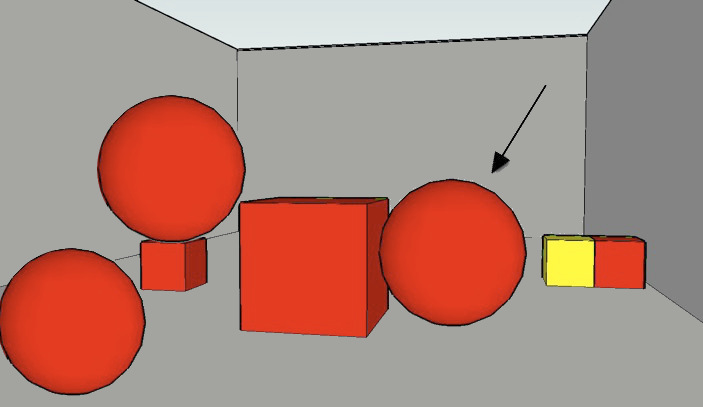
\includegraphics[width=.6\textwidth]{images/22paraRelacional.jpg}
\caption{Ejemplo de target.}
\label{target_mapa_3ball}
\end{figure}



Se cumple que  $e_1 \simil{\+L} e_5$, $e_3 \simil{\+L} e_5$ y $e_1 \simil{\+L} e_3$ ya que para toda f\'omula $\phi$, la {\bf interpretaci\'on de la f\'ormula} ($\interp \phi$) es $\{e_1, e_3, e_5\}$. 
$\phi_1$: $\nRed \land \nBall$ tenemos que $\interp {\phi_1} $= $\{e_1, e_3, e_5\}$

$\phi_2$: $\nLarge \land \nBall$, $\interp {\phi_2} $ = $\{e_1, e_3, e_5\}$

$\phi_3$: $\nRed \land \nLarge \land \nBall$, $\interp {\phi_3}$ = $\{e_1, e_3, e_5\}$

Esto nos dice que con ese lenguaje elegido $\+L$ la tarea GER con target $e_5$ no tiene soluci\'on.

La noci\'on de $\+L$-similaridad entonces, nos permite manejar el problema de  $\+L$-GER.
Por otra parte, podemos reformular esta de noci\'on de una manera estructural, para no considerar infinitas $\+L$-f\'ormulas y poder decidir si $u$ es $\+L$-similar a $v$. Podemos reinterpretar $\+L$-similaridad en t\'erminos de nociones de teor\'ia de modelos est\'andares
como isomorfismos o bisimulaciones que describen las propiedades estructurales de los modelos. Dados dos modelos$\tup{\Delta_1, \interp{\cdot}_1}$ y $\tup{\Delta_2,
\interp{\cdot}_2}$, considere las siguientes
propiedades de una relaci\'on binaria ${\sim} \subseteq \Delta_1 \times \Delta_2$ 
(vamos a considerar s\'olo modelos relacionales con relaciones unarias y binarias, ---es decir grafos etiquetados--- Usaremos $p$ para s\'imbolos unarios es decir proposicionales, y $r$ para s\'imbolos de relaciones binarias):
%(cf.~Convention~\ref{conv:signature}):
\smallskip 

\newcommand{\simdef}[2]{\noindent\ \ #1\hfill:\ \parbox[t]{.87\textwidth}{#2}\par}

\simdef{$\atomL$}{If $u_1{\sim} u_2$, entonces $u_1 \in \interp{p}_1 \Rightarrow u_2 \in \interp{p}_2$}
\simdef{$\atomR$}{If $u_1{\sim} u_2$, entonces $u_2 \in \interp{p}_2 \Rightarrow u_1 \in \interp{p}_1$}
\simdef{$\zig$}{If $u_1{\sim} u_2$ y $(u_1,v_1) \in \interp{r}_1$, entonces $\exists v_2$ tal que\ $v_1{\sim}v_2$
  y $(u_2,v_2) \in \interp{r}_2$}
\simdef{$\zag$}{If $u_1{\sim}u_2$ y $(u_2,v_2) \in \interp{r}_2$, entonces $\exists v_1$ tal que\ $u_1{\sim}v_1$ y
 $(u_1,v_1) \in \interp{r}_1$}
\simdef{$\injL$}{$\sim$ es una funci\'on inyectiva (cuando es restringida a su dominio)}
\simdef{$\injR$}{$\sim^{-1}$ es una funci\'on inyectiva (cuando es restringida a su dominio)}
\smallskip

Diremos que una relaci\'on binaria no vac\'ia $\sim$ es una 
{\bf $\+L$-simulaci\'on} cuando satisface las propiedades indicadas
en la Tabla~\ref{tab:simuls}. Por ejemplo, una relaci\'on binaria no vac\'ia que satisface $\atomL$, y $\zig$ es una $\EL$-simulaci\'on, como es indicado en fila~4 de la Tabla~\ref{tab:simuls}. M\'as a\'un, diremos que un objeto
{\bf $v$ $\+L$-simula $u$} ($u \simul{\+L} v$) si hay una relaci\'on $\sim$ que satisface la correspondiente propiedad tal que
$u \sim v$. El siguiente es un resultado fundamental del modelo te\'orico:%~\cite{ebbi:math96,KR99,BRV01}

\begin{table}[t]

\begin{tabular}{|l|l|cccccc|l|}
\hline
  $\+L$ & Descripci\'on &$\atomL$ & $\atomR$ & $\zig$ & $\zag$ & $\injL$ & $\injR$ & Comp.\\
  \hline
  $\FOL$ & (l\'ogica de primer orden)  & $\times$ & $\times$ & $\times$ & $\times$ & $\times$ & $\times$ & NP\\ \hline
  $\EPFOL$ & ($\FOL$ sin negaci\'on) & $\times$ & & $\times$ && $\times$ & & NP\\ \hline 
  $\ALC$   & ($\FOL$ sin desigualdad) & $\times$ & $\times$ & $\times$ & $\times$&& & P\\ \hline
  $\EL$   & ($\ALC$ sin negaci\'on) & $\times$ & &  $\times$ & & & &P\\ \hline
	$\ELUNEG$ & ($\EL$ m\'as disyunci\'on y  & $\times$ & $\times$ &  $\times$ & & & &P\\ 
	&negaci\'on proposicional)&&&&&&&\\ \hline
  $\ELAN$ & ($\EL$ con negaci\'on & $\times$ & $\times$ &  $\times$ & & & &P\\ 
	&proposicional) &&&&&&& \\ \hline
	$\PL$ & ($\ALC$ sin existencial --- & $\times$ & $\times$ & & & & &P\\ 
	&conj. dis. neg. prop.)&&&&&&&\\ \hline
	$\CL$ & (prop. conj. sin negaci\'on)& $\times$ &  &  & & & &P\\ 
	
\hline	
\end{tabular}

\caption{$\+L$-simulaciones para varios lenguajes l\'ogicos.}\label{tab:simuls}
\end{table}

\newtheorem{teorema}{Teorema}
%$Una l\'ogica sim\'etrica cumple  $\atomL$ y $\atomR$ como se ve en la Tabla \ref{tab:simuls}. 
\begin{teorema} \label{thm:simulation}
Si  $\+M_1 = \tup{\Delta_1, \interp{\cdot}_1}$ y $\+M_2 =
\tup{\Delta_2, \interp{\cdot}_2}$ son modelos finitos, $u \in
\Delta_1$ y $v \in \Delta_2$, entonces $u \simil{\+L} v$ si y s\'olo si $u
\simul{\+L} v$ (para $\+L \in \cset{\FOL,\EPFOL,\ALC,\EL,\ELAN}$).
\end{teorema}
%\begin{proof}
Algunos resultados son bien conocidos: $\simul{\FOL}$ es isomorfismo en
grafos etiquetados~\cite{ebbi:math96}; $\simul{\ALC}$ corresponde a la
noci\'on de bisimulaci\'on~\cite[Def.~2.16]{BRV01}; $\simul{\EL}$ es una
simulaci\'on definida en~\cite[Def.~2.77]{BRV01}. Los restantes son variaciones de estos.
%\end{proof}

Por lo tanto, en los modelos finitos\footnote{Que el modelo sea finito no es la hip\'otesis m\'as d\'ebil,
pero es suficiente para nuestro desarrollo.}, las simulaciones capturan exactamente el concepto de similaridad.
La implicaci\'on de derecha a izquierda no se mantiene en general sobre modelos infinitos.

Las $\+L$-simulaciones nos permiten determinar, de una manera eficaz,
cuando un objeto no se puede distinguir de otro en un modelo dado con respecto a $\+L$.

Por ejemplo, podemos probar que $a \simul{\EL} b$ en el modelo de la 
Figura~\ref{fig:cat-dog-1} ya que la relaci\'on ${\sim} = \{(a,a), (a, b) \}
%\cup\{ (x,x) \mid x \in \Delta\}
$ satisface $\atomL$ y $\zig$.
Usando el Teorema~\ref{thm:simulation} conclu\'imos que no hay
 \EL-descripci\'on para $a$, desde que para cualquier \EL-f\'ormula $\gamma$,
si $a\in\interp{\gamma}$, entonces $b\in\interp{\gamma}$.
Observe que $b \not\simul{\EL} a$, desde que
(aplicando de nuevo el Teorema~\ref{thm:simulation}), $b\in\interp{\aSmall(x)}$ pero
$a\notin\interp{\aSmall(x)}$.
%

Si se opta por un lenguaje m\'as rico que $\EL$, tal como $\ELAN$, uno puede ser
capaz de describir a $a$: toma, por ejemplo, la f\'ormula de $\ELAN$
$\nDog(x)\wedge\lnot\aSmall(x)$.

En la Tabla \ref{tab:algoritmosLogicas} se muestra un listado de algoritmos del \'area y la l\'ogica que cada uno de ellos usa para generar ER.
\begin{table}[h!]
\begin{tabular}{l|l}
  Algoritmo de GER & Variante de L\'ogica de Descripci\'on (LD)\\
  \hline
	  Full brevity & $\CL$ (proposicionales y conjunciones --- sin negaci\'on) \\
		Heur\'istica Greedy & $\CL$ (proposicionales y conjunciones --- sin negaci\'on) \\
  Incremental - Dale and Reiter (1995) & $\CL$ (proposicionales y conjunciones --- sin negaci\'on) \\
  GRAPH - van Deemter (2002) & $\PL$ (f\'ormulas conjuntivas, disjuntivas, negativas prop. \\
														& ---l\'ogica proposicional idem $\ALC$ sin existencial)\\
  Relacional - Dale and Haddock (1991)   & $\EL$ (Conjunciones de f\'ormulas, existenciales de f\'ormulas, \\
	& y proposicionales)\\
  Kelleher and Kruijff (2006)   & $\EL$ \\
  Gardent (2002) & \ELUNEG ($\EL$ m\'as disyunci\'on y negaci\'on proposicional)\\
\end{tabular}
\caption{Algoritmos y sus l\'ogicas asociadas.}\label{tab:algoritmosLogicas}
\end{table}


Como veremos en la siguiente subsecci\'on, la simulaci\'on nos d\'a un
enfoque eficiente, computacionalmente factible para atacar el problema $\+L$-GER. Algoritmos para calcular muchos tipos de $\+L$-simulaciones son
bien conocidos (vea, \cite{H71,areces08,HHK95,DPP03}), y para muchos
lenguajes (por ejemplo, \ALC, \ALC con negaci\'on de relaciones, \ELAN y \EL)
se ejecutan en tiempo polinomial (por otro lado, es conocido que no hay algoritmo polinomial 
 para simulaci\'on con \FOL- o \EPFOL, incluso la exacta
complejidad del problema en estos casos est\'a abierta \cite{gare:comp79}).

\section{GER v\'ia conjuntos de simulaci\'on}\label{sec:simulation}
\label{sec:greViaSimulacion}
En esta secci\'on discutiremos como resolver el problema $\+L$-GER
usando simulaci\'on. Dado un modelo $\+M = \tup{\Delta,
\interp{\cdot}}$, el Teorema~\ref{thm:simulation} nos dice que si 2 elementos distintos $u$ y $v$ en $\Delta$ son tales que $u
\simul{\+L} v$ entonces para toda $\+L$-f\'ormula que es verdadera para $u$ es tambi\'en verdadera para $v$. No hay f\'ormula en $\+L$ que pueda identificar un\'ivocamente a $u$. Desde esta perspectiva, conociendo cuando el modelo contiene un elemento que es $\gL$-similar pero distinto de $u$ es
equivalente a decidir si hay una expresi\'on referencial en $\+L$ para $u$.


Asumamos un lenguaje fijo $\+L$ y un modelo $\+M$. Supongamos que queremos referirnos a un elemento $u$ del dominio de $\+M$. Queremos computar el {\bf conjunto de simulaci\'on} de $u$ definido como
$\simset_{\+L}^{\+M}(u) = \cset{v \in \Delta \mid u \simul{\+L} v}$.
Cuando un modelo $\+M$ es claro de el contexto, simplemente escribimos $\simset_{\+L}$.
 Si $\simset_{\+L}^{\+M}(u)$ no es singleton $\cset{u}$,
el problema $\+L$-GER con target $\{u\}$ en $\+M$ fallar\'a.

%\iffullversion
%Es facil de ver que la union de 2 $\+L$-simulaciones 
%es tambi\'en una $\+L$-simulation. Podemos entonces definir el \emph{maximal
%auto $\+L$-simulation} (notaci\'on, $\simmax_{\+L}$) sobre un modelo $\+M$ como la union de todos los
%auto $\+L$-simulations sobre $\+M$. Ya que
%$\simset_{\+L}(u) = \cset{v \mid u \simmax_{\+L} v}$, un algoritmo
%para computar $\simmax_{\+L}$ tambi\'en computa $\simset_{\+L}(u)$.
%\else
%\fi
%
%\iffullversion
%Si $P$ es reflexiva y transitiva entonces tambi\'en lo es $\simmax_P$. En
%particular, $\simmax$ es reflexiva y transitiva.
%%\fixme{Are reflexivity and transitivity important? Check.}
%\else
%\fi



Un algoritmo para computar $\simset_{\ELAN}(v)$ es dado en~\cite{HHK95}. Para cada
elemento $v$ de un modelo dado finito
$\+M=\tup{\Delta,\interp{\cdot}}$
%\footnote{%
%  Actually the algorithm proposed in \cite{HHK95} is over labeled graphs, but
%  it can be adapted to compute $\simset_{\ELAN}$ by
%  appropriately labeling the model.%
%}
computa en tiempo $O(\size{\Delta}\times\size{{\interp{\cdot}}})$.
Intuitivamente, este algoritmo
define $S(v)$ como un conjunto de candidatos para simular $v$ y
sucesivamente refina este conjunto borrando aquellos elementos los cuales fallan en simular $v$.
%Since we never put new vertices into $\simset(v)$, all the deletions
%from $\simset(v)$ are permanent.
Al final, $S(v)=\simset_\ELAN(v)$. El algoritmo puede ser adaptado para
computar $\simset_\+L$ para cualquier otro languaje $\+L$. En particular,
lo podemos usar para computar $\simset_\EL$ en tiempo polinomial y nos dar\'a un l\'imite superior a la
complejidad del algoritmo b\'asico para establecer un l\'imite superior a la complejidad de el problema \EL-GER 
--esto responder\'ia la pregunta abierta~\cite{areces08}. El pseudo-c\'odigo es mostrado en el
Algoritmo~\ref{alg:schematic-gen-sim}, el cual usa la siguiente
notaci\'on: $\+P$ es un conjunto fijo de s\'imbolos de relaciones unarias, para $v\in
\Delta$, sea $\unary(v)=\{p\in\+P\mid v\in\interp{p}\}$ y sea tambi\'en
$\su{r}{v}=\{u\in\Delta\mid(v,u)\in\interp{r}\}$ para $r$ un s\'imbolo de relaci\'on binaria.

La Figura \ref{target_mapa_3ball} no pertenece al corpus GRE3D7, fue intencionalmente modificada para mostrar un caso en el que las propiedades proposicionales no alcanzan para dar una ER del objeto se\~nalado por la flecha. Para esa figura el algoritmo podr\'ia empezar con $S(v)$ = large, red, ball y luego el \'unico sucesor ser\'ia el red cube con la relaci\'on right-of, lo cual borra los dem\'as distractores.

%\newtheorem{algoritmo}{Algoritmo}
%%ROMI



%\floatname{algorithm}{Procedure}
\begin{algorithm}
\floatname{algorithm}{Algoritmo}
\small
\caption{ Computando \EL-similaridad\label{alg:schematic-gen-sim}}
%\captionsetup[algorithm]{name=Algoritmo}
\SetKwInOut{Input}{input}\SetKwInOut{Output}{output}
\Input{un modelo finito $\+M=\tup{\Delta,\interp{\cdot}}$}
\Output{$\forall v\in \Delta$, el conjunto de simulaciones
$\simset_\EL^{\+M}(v)=S(v)$} \BlankLine

\ForEach{$v\in \Delta$}{$S(v):=\{u\in \Delta \mid \unary(v)
\subseteq \unary(u) \}$}

\While{\guard}{$S(u):=S(u)\setminus\{w\}$}
\end{algorithm}


%First some notation. For any $v\in \Delta$ and any binary relation
%$r$, let
%\begin{eqnarray*}
%\unary(v)&=&\{p\mid \mbox{$p$ is a unary rel.\ and
%$v\in\interp{p}$}\}\\
%%\pr{r}{v}&=&\{u\in\Delta\mid(u,v)\in\interp{r}\}\\
%\su{r}{v}&=&\{u\in\Delta\mid(v,u)\in\interp{r}\}
%\end{eqnarray*}
%%The last two extend to sets $V\subseteq\Delta$ as usual:
%%$\pr{r}{V}=\bigcup_{v\in V}\pr{r}{v}$ and $\su{r}{V}=\bigcup_{v\in
%%V}\su{r}{v}$.

%

%The algorithm is fairly straightforward. We initialize $S(v)$ with
%the set of all elements $u\in\Delta$ such that $\unary(v)\subseteq
%\unary(u)$, i.e., the set of all elements satisfying at least the
%same unary relations as $v$ (this guarantees that property $\atomL$ holds).
%At each step, if there are three elements $u$, $v$ and $w$ such that
%for some relation $r$, $(u,v) \in \interp{r}$, $w\in S(u)$
%(i.e., $w$ is a candidate to simulate $u$) but $\su{r}{w}\cap S(v) = \emptyset$
%(there is no element $w'$ such that $(w, w') \in \interp{r}$
%and $w'\in S(v)$) then clearly condition $\zig$ is not satisfied
%under the supposition that $\simset_\EL=S$. $S$ is `too big' because
%$w$ cannot simulate $u$. Hence $w$ is removed from $S(u)$.

Inicializamos $S(v)$ con
el conjunto de todos los elementos $u\in\Delta$ tal que $\unary(v)\subseteq
\unary(u)$, es decir, el conjunto de todos los elementos que cumplan al menos las
mismas relaciones unarias que $v$ (esto garantiza que la propiedad $\atomL$ se mantiene).
En cada paso, si hay tres elementos $u$, $v$ y $w$ tales que
por alguna relaci\'on $r$, $(u,v) \in \interp{r}$, $w\in S(u)$
(Es decir, $w$ es un candidato para simular $u$) pero $\su{r}{w}\cap S(v) = \emptyset$
(No hay ning\'un elemento $w'\in S(v)$) tal que $(w, w') \in \interp{r}$
y $w'\in S(v)$) entonces es claro que la condici\'on $\zig$ no se cumple
bajo la suposici\'on de que $\simset_\EL=S$. $S$ es 'demasiado grande' porque
$w$ no puede simular $u$. Por lo tanto $w$ se borra de $S(u)$.


El Algoritmo~\ref{alg:schematic-gen-sim} nos dir\'a cuando hay una expresi\'on referencial en \EL (\EL-ER) para alg\'un elemento $u$ (esto es, cuando
$\simset_{\EL}(u) = \cset{u}$ o no). No computa ninguna \EL-f\'ormula $\varphi$ que identifique \'univocamente a $v$. Pero
podemos adaptarlo para obtener tal f\'ormula.
La estrategia principal del Algoritmo~\ref{alg:schematic-gen-sim} para computar simulaciones es sucesivamente refinar una aproximaci\'on al conjunto de simulaci\'on.
%is to successively
%refine an over-approximation of the simulator sets.
La ``raz\'on'' detr\'as de cada refinamiento puede ser codificada usando una \EL-f\'ormula.
%Using this insight, 
Uno puede transformar un algoritmo que computa un conjunto de $\+L$-simulaci\'on con una estrategia similar, en uno que adem\'as compute una $\+L$-ER para cada conjunto.


El Algoritmo~\ref{alg:schematic-GRE} muestra una versi\'on transformada del 
Algoritmo~\ref{alg:schematic-gen-sim}. La idea es que cada nodo
$v\in\Delta$ es ahora etiquetado con una f\'ormula
$F(v)$ de \EL. Las f\'ormulas $F(v)$ son actualizadas a trav\'ez de la ejecuci\'on del ciclo cuyo invariante asegura que $v \in
\interp{F(v)}$ y $\interp{F(u)} \subseteq S(u)$ se mantienen para
$u,v\in\Delta$.

%\begin{algorithm}
%\small
%%\LinesNumbered
%\io
%
%\ForEach{$v\in \Delta$}
%{ 
		%$S(v):=\{u\in \Delta \mid \unary(v) \subseteq \unary(u) \}$ \label{alg:line:init1}
%
		%$F(v):=\bigwedge \unary(v)$ \label{alg:line:init2}
%}
%
%\While{\guard}
%{
 %%$\{\ I: \mbox{\bf assert }(\forall u,v)\ \interp{F(u)} \subseteq S(u)\wedge v \in \interp{F(v)} \ \}$
 %\KwSty{invariant} $\forall u,v: \interp{F(u)} \subseteq S(u)\wedge v \in \interp{F(v)}$\\
%$S(u):=S(u)\setminus\{w\}$\;\label{alg:line:loop-body-begin}
%
%\If{$\diam F(v)$ is not a conjunct of $F(u)$}
	%{ 
		%$F(u):=F(u)\wedge \diam F(v)$ \label{alg:line:loop-body-end-1} 
	%}
%} \caption{\small Computing $\EL$-similarity and \posre} 
%\label{alg:schematic-GRE}
%\end{algorithm}


%%ESTE TRADUCIDO!!!
\begin{algorithm}\small
\floatname{algorithm}{Algoritmo}
%\LinesNumbered
\io

\ForEach{$v\in \Delta$}{ $S(v):=\{u\in \Delta \mid \unary(v)
\subseteq \unary(u) \}$ \label{alg:line:init1}

$F(v):=\bigwedge \unary(v)$ \label{alg:line:init2} }

\While{\guard}
{
 %$\{\ I: \mbox{\bf assert }(\forall u,v)\ \interp{F(u)} \subseteq S(u)\wedge v \in \interp{F(v)} \ \}$
 \KwSty{invariante} $\forall u,v: \interp{F(u)} \subseteq S(u)\wedge v \in \interp{F(v)}$\\
$S(u):=S(u)\setminus\{w\}$ \label{alg:line:loop-body-begin}

\If{$\diam F(v)$ no es conjunci\'on de $F(u)$}{ $F(u):=F(u)\wedge
\diam F(v)$ \label{alg:line:loop-body-end-1} }} \caption{\small
Computando $\EL$-similaridad y \posre}\label{alg:schematic-GRE}
\end{algorithm}

Inicialmente $F(v)$ es la conjunci\'on de todas las relaciones unarias que
satisfacen $v$ (si no hay ninguna, entonces $F(v)=\top$).
el algoritmo busca elementos $r,u,v,w$ tales que
$(u,v)\in\interp{r}$, $w\in S(u)$ y $\su{r}{w}\cap
S(v)=\emptyset$, actualiza $F(u)$ a $F(u)\wedge\diam F(v)$.
De nuevo, \'esta nueva f\'ormula $\phi$ est\'a en $\pos$ y se puede mostrar que
$v\in\interp{\phi}$ y $w\notin\interp{\phi}$, por lo tanto hay testigos de que $v\simil{\EL} w$ es falso.

%As we will see in Theorem~\ref{thm:correctness-schematic-GRE}, this
%formula is true in $v$ but false in $w$, hence witnessing that $w$
%does not simulate $v$.


%It is clear that Algorithm \ref{alg:schematic-GRE} terminates.
%
%\iffullversion One wants to know whether a given set $V\subseteq W$
%has an \posre. How do we interpret the output of Algorithm
%\ref{alg:schematic-GRE}? Here is the answer: $V\subseteq W$ has an
%\EL-RE iff there is a node $v\in V$ such that $V=\{u\in W\colon
%v\in\simset_\subseteq(u) \wedge u\in\simset_\subseteq(v)\}$. In
%other words, $V$ has an \EL-RE iff $V$ is the set of nodes which are
%\emph{bisimilar} to some node of $V$. Here we say that $u$ and $v$
%are \emph{bisimilar} if $u\in\simset_\subseteq(v)$ and
%$v\in\simset_\subseteq(u)$. In case $V=\{v_1,\dots,v_n\}$ has an
%\posre, any $F(v_i)$ is a valid \posre, so one can pick any of them.

\iffullversion Uno quiere saber si un determinado conjunto  $V\subseteq W$
tiene un \posre. ¿C\'omo interpretar la salida del algoritmo
\ref{alg:schematic-GRE}`? Aqu\'i est\'a la respuesta: $V\subseteq W$ tiene una
\EL-RE si y s\'olo si hay un nodo $v\in V$ tal que  $V=\{u\in W\colon
v\in\simset_\subseteq(u) \wedge u\in\simset_\subseteq(v)\}$. En
Es decir, $V$ tiene un \EL-RE si y s\'olo si $V$ es el conjunto de nodos que son
\emph{bisimilar} a alg\'un nodo de $V$. Aqu\'i decimos que $u$ y $v$
son \emph{bisimilar} si $u\in\simset_\subseteq(v)$ y
$v\in\simset_\subseteq(u)$. En caso  $V=\{v_1,\dots,v_n\}$ tiene una
\posre, ninguna $F(v_i)$ es un \posre v\'alida, por lo que uno puede elegir cualquiera de ellas.

%
%In particular, $v$ has an \EL-RE if and only if $\simset_\subseteq(v)=\{v\}$
%and in case $v$ has a \EL-referring expression then $F(v)$ is a
%valid one. If $v$ does not have an \posre then the algorithm may be
%used to approximate an \posre. Indeed, since every formula true at
%$v$ is also true at all nodes in $\simset_\subseteq(v)$ and $F(v)$
%is true at every node of $\simset_\subseteq(v)$ then $F(v)$ is a
%reasonable approximation of an \EL-RE for $v$.

En particular, $v$ tiene un \EL-ER si y s\'olo si $\simset_\subseteq(v)=\{v\}$
y en caso de $v$ tiene una expresi\'on \EL-expresi\'on referencial, $F(v)$ es una v\'alida. Si $v$ no tiene un \posre entonces el algoritmo puede ser
utilizado para aproximar una \posre. De hecho, ya que cada f\'ormula en cierta en $v$
tambi\'en es cierto en todos los nodos de $\simset_\subseteq(v)$ y $F(v)$
es cierto en todos los nodos de $\simset_\subseteq(v)$ entonces $F(v)$ es una
aproximaci\'on razonable de un \EL-RE por $v$.

\begin{ex}
Sea $\gG$ el siguiente modelo
\begin{center}
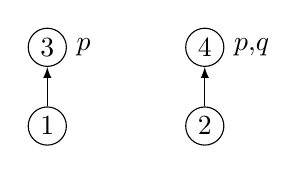
\begin{tikzpicture}[>=latex]
  \node (n1) at (0,0) [shape=circle,draw,inner sep=2pt, label=right:$$] {$1$} ;
  \node (n2) at (2,0) [shape=circle,draw,inner sep=2pt, label=right:$$] {$2$} ;
  \node (n4) at (0,1) [shape=circle,draw,inner sep=2pt, label=right:$p$] {$3$} ;
  \node (n5) at (2,1) [shape=circle,draw,inner sep=2pt, label=right:$p{,}q$] {$4$} ;
  \draw [->] (n1) -- (n4);
  \draw [->] (n2) -- (n5);
\end{tikzpicture}
\end{center}
%
donde $\rg\ l=\cset{p,q}$ y la valuaci\'on es definida como
$l(3)=\cset{p}, l(4)=\cset{p,q}, l(1)=l(2)=\cset{}$. Los valores iniciales de $S$ y $F$ son los que se muestran en
Tabla~\ref{tab:example}.

\begin{table}[ht]
\centering
{\footnotesize
\begin{tabular}{|c|c|c|c|c|}
\hline
&\multicolumn{2}{|c|}{Initial}&\multicolumn{2}{|c|}{Final}\\
$v$ & $S(v)$ & $F(v)$ & $S(v)$&$F(v)$\\
\hline
$1$ & $\{1,2,3,4\}$ & $\top$ & $\{1,2\}$&$\top\wedge\diam p$\\
$2$ & $\{1,2,3,4\}$ & $\top$ & $\{2\}$&$\top\wedge\diam(p\wedge q)$\\
$3$ & $\{3,4\}$ & $p$ & $\{3,4\}$ &$p$\\
$4$ & $\{4\}$ & $p\wedge q$ & $\{4\}$&$p\wedge q$\\
\hline
\end{tabular}
\caption{Valores iniciales y finales de $F$ y $S$}\label{tab:example}
}
\end{table}

Supongamos la siguiente ejecuci\'on:
\begin{enumerate}
\item Elegir $u=2,v=4,w=1$: detect that $1$ no simula $2$; set $S(2)=\{2,3,4\}$ y $F(2)=\top\wedge\diam(p\wedge q)$
\item Elegir $u=2,v=4,w=3$: detecta que $3$ no simula $2$; set $S(2)=\{2,4\}$ y $F(2)=\top\wedge\diam(p\wedge q)$
\item Elegir $u=2,v=4,w=4$: detecta que $4$ no simula $2$; set $S(2)=\{2\}$ y $F(2)=\top\wedge\diam(p\wedge q)$
\item Elegir $u=1,v=3,w=3$: detecta que $3$ no simula $1$; set $S(1)=\{1,2,4\}$ y $F(1)=\top\wedge\diam p$
\item Elegir $u=1,v=3,w=4$: detecta que $4$ no simula $1$; set $S(1)=\{1,2\}$ y $F(1)=\top\wedge\diam p$
\end{enumerate}
%After the fifth iteration it terminates. The final output is shown
%in Table~\ref{tab:example}. From this output one may conclude that,
%since $\simset_\subseteq(4)=\{4\}$, node $4$ has an \posre, namely
%$p\wedge q$. Node $2$ also has the \EL-RE $\top\wedge\diam(p\wedge
%q)$. In contrast $3$ does not have an \EL-RE because every
%$\pos$-formula true at $3$ is also true at $4$ (in this case, the
%only such possible formula is $p$ itself, or logically equivalent
%formulas such as $\top\wedge p\wedge p$). Nor $3$ has an \posre.

Despu\'es de la quinta iteraci\'on termina. Se muestra el resultado final
En la Tabla~\ref{tab:example}. A partir de esta salida se puede concluir que,
ya que$\simset_\subseteq(4)=\{4\}$, el nodo $4$ tiene un \posre, a saber,
$p\wedge q$. Nodo $2$ tambi\'en tiene la \EL-RE $\top\wedge\diam(p\wedge
q)$. En contraste $3$ no tiene un \EL-RE, porque cada
$\pos$-f\'ormula verdadera en $3$ tambi\'en es cierta en $4$ (en este caso, el
S\'olo tales f\'ormula posible es $p$ en s\'i mismos o equivalentes
f\'ormulas como $\top\wedge p\wedge p$). Tampoco $3$ tiene un \posre.

\end{ex}
\fi

\iffullversion
\begin{theorem}\label{thm:correctness-schematic-GRE}
Sea $S$ y $F$ la salida del Algoritmo
\ref{alg:schematic-GRE} con input $\gG=\tup{N,\to,l}$. Entonces para cada
nodo $v\in N$, $\interp{F(v)} = S(v) = \simset_\subseteq(v)$
\end{theorem}
\fi

\iffullversion
\begin{proof}
Es claro que para cada nodo $v\in N$,
$\simset_\subseteq(v)=S(v)$. Para la segunda parte, proponemos el siguiente invariante en el loop principal:
\begin{itemize}
\item[$I_1$:] para cada $v\in N$, $v \in \interp{F(v)}$
\item[$I_2$:] para cada $u,v\in N$, $\interp{F(u)} \subseteq S(u)$
\end{itemize}

Vamos a analizar el estado despu\'es de la inicializaci\'on, antes de la l\'inea~\ref{alg:line:loop-begin} se ejecuta por primera vez. En el uno
parte, es claro que para cualquier nodo $v\in N$, $v \in \interp{F(v)}$, as\'i
$I_1$ es verificado. Por otro lado, si $v\notin S(u)$ entonces
$l(u)\not\subseteq l(v)$ y hay un s\'imbolo proposicional $p$ tal que $p \in l(u)$ y $p \notin l(v)$. Desde que $v\notin\interp{p}$
entonces $v\notin\interp{\bigwedge l(u)}$ y as\'i
$v\notin \interp{F(u)}$.

Supongamos que $I_1$ y $I_2$ son verdaderos antes de ejecutar la 
l\'inea~\ref{alg:line:loop-body-begin}. Para todo $v\in N$ sea $S(v)=S_v$ y
$F(v)=\phi_v$ en este estado. Sean $u,v,w$ los nodos elegidos. Mostramos que el invariante es reestablesido luego de ejecutar la l\'inea
\ref{alg:line:loop-body-end-1}. Desde que $F$ y $S$ s\'olo cambian para $u$, 
es suficiente mostrar
\begin{itemize}
\item[$I_1'$:] $u \in \interp{\phi_u\wedge\diam \phi_v}$
\item[$I_2'$:] $\forall v\in N, \interp{\phi_u\wedge\diam \phi_v} \subseteq S_u\setminus\{w\}$
\end{itemize}
Para$I_1'$, es claro de $I_1$ que $u \in \interp{\phi_u}$ y $v \in \interp{\phi_v}$. Desde que $u\to v$ conclu\'imos que $u \in \interp{\diam
\phi_v}$.

Para $I_2'$ mostramos que para cualquier $v$, si $v\notin S_u\setminus\{w\}$
entonces $v\notin \interp{\phi_u\wedge\diam \phi_v}$. Si $v\notin S_u$,
por $I_2$ conocemos que $v\notin \interp{\phi_u}$ y entonces $v\notin
\interp{\phi_u\wedge\diam \phi_v}$. Supongamos que $v=w$ y, por
contradicci\'on, asumimos $v \in \interp{\phi_u\wedge\diam \phi_v}$.
Hay $w'\in N$ tal que $v\to w'$ y $w' \in
\interp{\phi_v}$. Por $I_2$ esto implica $w'\in S_v$. Aqu\'i $w'\in\su(w)\cap S_v$ y esto contradice la elecci\'on de $u,v,w$.

Cuando el algoritmo termina, $S=\simset_\subseteq$ y
el invariante $I_2$ implica que para cada $u,v\in N$,
$F(u) \subseteq \simset_\subseteq(u)$. Por otro lado, $I_1$
implica que $u \in \interp{F(u)}$ y por Proposici\'on \ref{prop:equiv} tenemos que si
 $v\in \simset_\subseteq(u)$ entonces $v \in \interp{F(u)}$.

Por lo tanto para cada $u,v\in N$, $\interp{F(u)} = \simset_\subseteq(u)$. 
As\'i que definiendo $\form:=F$ obtenemos el resultado deseado.
\end{proof}
\else
\fi

\iffullversion
\begin{theorem}
Algoritmo~\ref{alg:schematic-GRE} con input $\gG = \tup{N,\to,l}$
termina en tiempo
$O(\size{{\to}}^2\cdot\size{N}^3+\size{N}\cdot\size{\rg\ l})$.
\end{theorem}
\fi

\iffullversion
\begin{proof}
Para una implementaci\'on ingenua, el bucle principal se ejecuta en la mayor\'ia $\size{N}^2$ 
muchos pasos y para encontrar $u,v,w$ en
la l\'inea~\ref{alg:line:loop-begin} necesitamos $O(\size{N}\cdot\size{{\to}}^2)$

muchos pasos. El tiempo de ejecuci\'on del cuerpo del bucle es absorbida por este
\'ultima cantidad. Por lo tanto, en el tiempo total de ejecuci\'on del bucle principal es $O(\size{{\to}}^2\cdot\size{N}^3)$. Para cada $v\in N$, necesitamos
$O(\size{\rg\ l})$muchos pasos para las l\'ineas~\ref{alg:line:init1} y~\ref{alg:line:init2}. 
As\'i que en total, la inicializaci\'on toma $O(\size{N}\cdot\size{\rg\ l})$ 
muchos pasos.
\end{proof}
\else
\fi

\iffullversion
\begin{algorithm} \floatname{algorithm}{Algoritmo}\small
\io

\ForEach{$v\in \Delta$}{ $\prevS(v):=\Delta$

\If{para toda $r$ binaria, $\su{r}{v}=\emptyset$}{$S(v):=\{u\in \Delta
\mid \unary(v)\ \subseteq \unary(u) \}$

$F(v):=\bigwedge\unary(v)$ } \Else{ sea $r$ una relaci\'on binaria tal que $\su{r}{v}\not=\emptyset$

 $S(v):=\{u\in \Delta \colon
\unary(v) \subseteq \unary(u)\wedge\su{r}{u}\not=\emptyset \}$

$F(v):=\diam\top\wedge\bigwedge P(v)$ }}

\While{$\exists\ v\in \Delta:S(v)\not=\prevS(v)$}{

$\{\ I_1:\mbox{\bf assert\ }(\forall v)\ S(v)\subseteq\prevS(v)\ \}$

$\{\ I_2:\mbox{\bf assert\ }(\forall r,u,v,w)\
[(u,v)\in\interp{r}\wedge w\in
S(u)]\Rightarrow[\su{r}{w}\cap\prevS(v)\not=\emptyset]\ \}$

\ForEach{\mbox{\rm relaci\'on binaria $r$ y $u\in \pr{r}{v}$}}{

$remove := \pr{r}{\prevS(v)}\setminus\pr{r}{S(v)}$

$S(u):=S(u)\setminus remove$

\If{$\diam F(v)$ no es conjunci\'on de $F(u)$}{ $F(u):=F(u)\wedge
\diam F(v)$\label{alg:line:loop-body-end-2} } }

$\prevS(v)=S(v)$

} \caption{\small refinado $\EL$-similaridad y
\posre}\label{alg:refined-GRE}
\end{algorithm}
\fi

Algoritmo \ref{alg:schematic-GRE} se puede modificar f\'acilmente para
calcular la \ELAN-RE de cada conjunto de simulaci\'on $\simset_{\ELAN}$ 
ajustando la inicializaci\'on: reemplazando $\subseteq$ por $=$ en la
inicializaci\'on de $S(v)$ e inicializando $F(v)$ como
$\bigwedge\left(\unary(v)\cup\overline \unary(v)\right)$,
donde $\overline \unary(v)=\{\lnot p\mid v\notin\interp{p}\}$.


Una implementaci\'on ingenua del Algoritmo~\ref{alg:schematic-GRE}
ejecuta en tiempo $O(\size{\Delta}^3\times$
$\size{\interp{\cdot}}^2)$
%\fixme{Santi: chequear la complejidad}
dando una soluci\'on polinomial a los problemas \EL y \ELAN-GER.
El Algoritmo~\ref{alg:schematic-gen-sim} puede ser transformado para ejecutar con a una menor complejidad como se muestra en
~\cite{HHK95}; m\'as a\'un \'esta versi\'on del algoritmo puede ser adaptada para
computar \EL- y \ELAN-RE para un subconjunto arbitrario del dominio de $\tup{\Delta,\interp{\cdot}}$
 en $O(\size{\Delta}\times\size{\interp{\cdot}})$ pasos. 


%Given $\gG = \tup{N,\to,l}$,
%the
%
%$F$, the set of \posre, and $S$, the simulator sets tal que\ $(\forall
%v\in \Delta)\ \interp{F(v)}=S(v)=\simset_\EL(v)$

%
\begin{theorem}\label{thm:complexity-EL-GRE}
Los problemas \EL y \ELAN-GER sobre $\gM=\tup{\Delta,\interp{\cdot}}$ tienen complejidad
$O(\size{\Delta}\times\size{\interp{\cdot}})$.
\end{theorem}

%Theorem~\ref{thm:complexity-EL-GER} answers a question left open
%in~\cite{AKS08}: the \EL-GER problem can be solved in polynomial
%time. Note, however, that this  result assumes a convenient representation of
%formulas like, for example, directed acyclic graphs, to ensure that
%each step of the formula construction can be done in $O(1)$. In
%\sect{size} we will take a closer look at the issue and its relation to
%the size of the smallest $\+L$-RE.


El Teorema~\ref{thm:complexity-EL-GRE} responde a una pregunta dejada abierta
en~\cite{areces08}: el problema \EL-GER se puede resolver en tiempo polinomial. N\'otese, sin embargo, que este resultado supone una representaci\'on conveniente de
f\'ormulas como, por ejemplo, grafos ac\'iclicos dirigidos, para asegurar que
cada paso de la construcci\'on de la f\'ormula puede hacerse en $O(1)$. %En
%\sect{size} vamos a echar un vistazo m\'as de cerca el tema y su relaci\'on con
%el tamaño de los m\'as pequeños $\+L$-RE.

%Theorem~\ref{thm:complexity-EL-GRE} shows that there are efficient
%GRE algorihtms for \EL and \ELAN; languages which are --as discussed
%in \sect{choosinglanguage}-- generally simple to realize. The
%methods presented here, together with previous results
%of~\cite{AKS08} indicate that algorithms for computing
%$\+L$-simulator sets can, in many cases, be adapted to solve the
%$\+L$-GRE problem at no extra complexity cost.

%
%Algorithm~\ref{alg:schematic-GRE} was obtained by adding formula annotations
%to a standard `\EL-simulation-minimization' algorithm. Given an
%$\+L$-simulation-minimization, we can typically adapt it in an analogous
%way to obtain an $\+L$-GRE algorithm.
%The obtained algorithm computes $\+L$-REs for \emph{every} element of the
%domain simultaneously.
%This will make it particularly suitable for applications with
%static domains requiring references to many objects.


El Algoritmo~\ref{alg:schematic-GRE} se obtuvo mediante la adici\'on de anotaciones de f\'ormulas
a un algoritmo est\'andar `minimizaci\'on de \EL-simulaciones'. Dada una minimizaci\'on de
$\+L$-Simulaci\'on, podemos adaptarlo normalmente en una an\'aloga
manera de obtener un algoritmo $\+L$-GER.
El algoritmo calcula obtenido $\+L$-ERs para \emph{todos} los elementos de la
dominio simult\'aneamente.
Esto har\'a que sea especialmente adecuado para aplicaciones con
dominios est\'aticos que requieren referencias a muchos objetos.

% but given its low complexity
%and the fact that termination is ensured (no risk of infinite regression, see~\cite{dale91:_gener_refer_expres_invol_relat}),
%it seems suitable for most applications.
 %Moreover, the algorithm can be adapted
%to dynamic domains by using techniques used to recompute simulations (see~\cite{saha:incre07}),
%so that only those RE that were affected by a change in the domain need to be
%recomputed.

Por otra parte, el algoritmo se puede adaptar
a los dominios din\'amicos mediante el uso de t\'ecnicas que se utilizan para volver a calcular las simulaciones (see~\cite{saha:incre07}),
de modo que s\'olo los RE que se ve afectada por un cambio en el dominio necesita ser
recalculado.

%We have not addressed so far other relevant issues of the
%GRE problem besides computational complexity. In particular,
%Algorithm~\ref{alg:schematic-GRE} pays no attention to the use of
%preferences among relations when generating an RE (i.e., preferring
%the selection of certain attributes over others, when possible).
%While there is room for improvement (e.g., making a weighted choice
%instead of the non-deterministic choice when choosing elements
%in the main loop of the algorithm), support for preferences is not
%one of the strong points of this family of algorithms.
%We consider algorithms with strong support for preferences in the following section.

No hemos abordado hasta el momento otras cuestiones relevantes de la
problema GER adem\'as de la complejidad computacional. En particular,
Algoritmo~\ref{alg:schematic-GRE} no presta atenci\'on a la utilizaci\'on de
preferencias entre las relaciones cuando se genera una ER (es decir, prefiriendo
la selecci\'on de ciertos atributos por encima de otros, cuando sea posible).
Si bien no hay margen de mejora (por ejemplo, hacer una elecci\'on ponderada
en lugar de la elecci\'on no determinista la hora de elegir los elementos
en el bucle principal del algoritmo), el apoyo para las preferencias no es
uno de los puntos fuertes de esta familia de algoritmos.
Consideramos algoritmos con un fuerte apoyo a las preferencias en la siguiente secci\'on.


\section{Bisimulaci\'on}
\label{sec:bisimulacion}

%Este algoritmo fue propuesto por %\cite{}

La idea es transformar el problema de GER al problema de computar una f\'ormula de l\'ogicas para la descripci\'on (DL) cuyos elementos que satisfagan la f\'ormula sea el target.% (o los elementos targets, en el caso de querer dar una ER para plurales aprovechando que una f\'ormula describe un conjunto que puede contener m\'as de un elemento).\\

A continuaci\'on daremos una introducci\'on a las l\'ogicas para la descripci\'on \alc y \el. Explicaciones m\'as detalladas sobre \alc y \el se ver\'an en el Cap\'itulo \ref{sec:intro_logica}.

\emph{F\'ormulas} (o \emph{conceptos}) $\varphi$ de $\alc$ son generadas por la siguiente gram\'atica:
$$
\varphi,\varphi' ::= \top \mid p \mid \neg \varphi \mid \varphi \sqcap \varphi'
\mid \exists R. \varphi
$$
donde $p$ es el conjunto de los s\'imbolos proposicionales \prop y $R$ es el de los s\'imbolos relacionales \rel. $\el$ es la parte sin negaci\'on de $\alc$.\\

Las f\'ormulas de ambos $\alc$ y $\el$ son interpretadas en modelos relacionales de primer orden $\gM = (\Delta,\interp{\cdot})$ donde
$\Delta$ es un conjunto no vac\'io y $\interp{\cdot}$ es una funci\'on de interpretaci\'on tal que:
$$
\begin{array}{ccl}
\interp{p} & \subseteq & \Delta  \mbox{ para $p \in \prop$}\\
\interp{R} & \subseteq & \Delta \times \Delta  \mbox{ para $R \in \rel$}\\
\interp{\neg \varphi} & = & \Delta - \interp{\varphi}\\
\interp{\varphi \sqcap \varphi'} & = & \interp{\varphi} \cap \interp{\varphi'}\\
\interp{\exists R.\varphi} & = & \{i \mid \mbox{para alg\'un } i', (i,i') \in \interp{R}\\
& & \mbox{ e } i' \in \interp{\varphi} \}.\\
\end{array}
$$

\begin{figure}[t]
\begin{center}
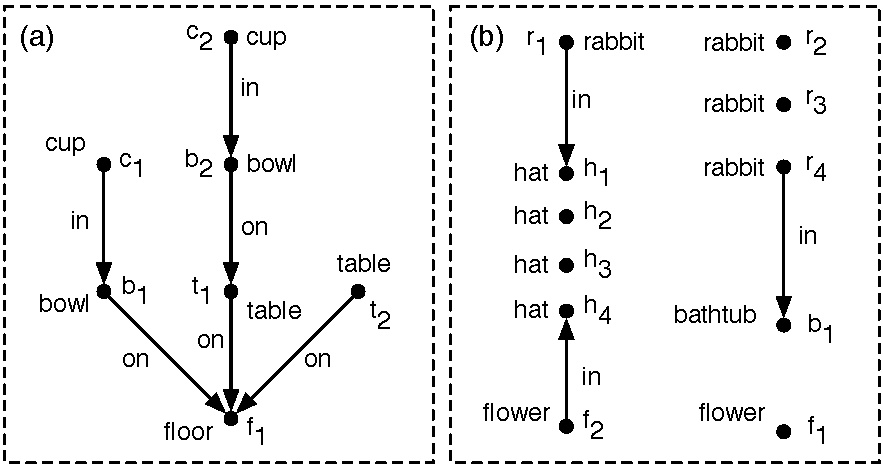
\includegraphics[width=8.5cm]{figures/pic-dale-haddock.pdf}\\[0pt]
\caption{}
\label{fig:dale-haddock}
\end{center}
\end{figure}


Cada f\'ormula de una descripci\'on l\'ogica denota un conjunto de objetos del dominio; por lo tanto podemos usar tales f\'ormulas para describir conjuntos. Por ejemplo en el modelo de la Figura.~\ref{fig:dale-haddock}b, la f\'ormula
$\mathsf{flower}$ denota el conjunto $\{f_1,f_2\}$; La f\'ormula
$\mathsf{flower} \sqcap \exists \mathsf{in}.\mathsf{hat}$ denota
$\{f_2\}$; y la f\'ormula $\mathsf{flower} \sqcap \neg
\exists \mathsf{in}.\mathsf{hat}$ denota $\{f_1\}$.\\

\textcolor{blue}{no se si dejar este ejemplo, o cambiarlo por uno es espa\~nol}

Hay muchas otras l\'ogicas de descripci\'on (DL) en la literatura por ejemplo 

$\mathcal{CL}$ (\el\ sin el cuantificador existencial, es decir solo conjunciones at\'omicas); $\mathcal{PL}$ (\alc\ l\'ogica propocisional); y
$\mathcal{ELU}_{(\neg)}$ (\el\ m\'as disjunci\'on y negaci\'on at\'omica).\\

Usaremos una noci\'on de preservaci\'on de f\'ormulas que llamaremos
\emph{similaridad}. Para cualquier DL $\gL$, diremos que un individual $i$ es \emph{\gL-similar} a $i'$ en un modelo dado $\gM$
si para cualquier f\'ormula $\varphi \in \gL$ tal que $i \in
\interp{\varphi}$, tambi\'en tenemos que $i' \in \interp{\varphi}$.\\
Equivalentemente, no hay $\gL$-f\'ormula que se mantenga para $i$ pero no para
$i'$.  Diremos que el \emph{\gL-conjunto de similaridad} de alg\'un individual
$i$ es el conjunto de todos los individuales a los cuales $i$ es \gL-similar.\\

Notar que la similaridad no es necesariamente una relaci\'on sim\'etrica: Por ejemplo:$f_1$ es \el-similar a $f_2$ en
Figura~\ref{fig:dale-haddock}b, pero $f_2$ no es \el-similar a $f_1$
(satisface la f\'ormula $\exists \mathsf{in}.\mathsf{hat}$ y $f_1$
no la satisface).  De todas maneras, \alc-similaridad es una relaci\'on sim\'etrica porque
el languaje contiene negaci\'on; y en consecuencia, $f_1$ no es \alc-similar
a $f_2$ porque este tampoco satisface $\neg \exists
\mathsf{in}.\mathsf{hat}$.  Porque \alc\ es m\'as expresivo que \el,
esto es, para alg\'un individual $a$ es posible ser \el-similar pero
no \alc-similar a alg\'un individual $b$, pero no viceversa.\\



%\textcolor{blue}{SACAR ESTO... poner quizas en la introduccion o en primer capitulo. Las ER que involucran relaciones han recibido m\'as atenci\'on recientemente;
%especialmente en el contexto de las expresiones referenciales espaciales en generaci\'on (por ejemplo,~\cite{kelleher06:increm}), donde es particularmente natural utilizar expresiones que implican relaciones espaciales, tales como ``la esfera en la parte superior del cubo''. Sin embargo, el algoritmo cl\'asico por~\cite{dale91:gener} ha demostrado ser incapaz de generar ER satisfactorias en la pr\'actica (v\'ease el an\'alisis sobre el~\emph{cabinet corpus} en~\cite{viethen06:_algor_for_gener_refer_expres}). Adem\'as, el Dale y Haddock algoritmo y muchos de sus sucesores (tales como~\cite{kelleher06:increm}) son vulnerables a el problema de la \emph{regresi\'on infinita}, donde el algoritmo entra en un bucle infinito, saltando hacia atr\'as y hacia adelante entre las descripciones para dos individuos emparentados, como en `` el libro sobre la mesa que soporta una libro sobre la mesa \ldots ''}

%REs involving relations have received increasing attention recently;
%especially in the context of spatial referring expressions in situated
%generation (e.g., \cite{kelleher06:increm}),
%where it is particularly natural to use expressions involving spatial
%relations such as ``the ball on top of the cube.''  However, the
%classical algorithm
%by~\cite{dale91:gener} was shown to be
%unable to generate satisfying REs in practice (see the analysis over
%the \emph{cabinet corpus}
%in~\cite{viethen06:_algor_for_gener_refer_expres}).  Furthermore, the
%Dale and Haddock algorithm and many of its successors (such
%as~\cite{kelleher06:increm}) are vulnerable to
%the problem of \emph{infinite regress}, where the algorithm enters an
%infinite loop, jumping back and forth between descriptions for two
%related individuals, as in ``the book on the table which supports a
%book on the table \ldots''

%\cite{arec2:2008:Areces,arec:usin11} have proposed low complexity
%algorithms for the generation of relational REs
%%(including references to sets) 
%that eliminate the risk of infinite regression.  These algorithms are
%based on variations of the partition refinement algorithms
%of~\cite{paig:thre87}.  The information provided by a given scene
%is interpreted as a relational model whose objects are classified into
%sets that fit the same description.  This classification is
%successively \emph{refined} till the target is the only element
%fitting the description of its class.  The existence of an ER depends
%on the information available in the input scene, and on the expressive
%power of the formal language used to describe elements of the
%different classes in the refinement.


\cite{arec2:2008:Areces,arec:usin11} han propuesto algoritmos de baja complejidad
 para la generaci\'on de ER relacionales que eliminan el riesgo de regresi\'on infinita. Estos algoritmos son
basados en variaciones de los algoritmos de refinamiento de particiones
de~\cite{paig:thre87}. La informaci\'on proporcionada por una escena dada
se interpreta como un modelo relacional cuyos objetos se clasifican en
conjuntos que se adaptan a la misma descripci\'on. Esta clasificaci\'on es
sucesivamente \emph{refinada} hasta que el target es el \'unico elemento
en la clase. La existencia de una ER depende
de la informaci\'on disponible en la escena de entrada, y del poder expresivo
del lenguaje formal utilizado para describir los elementos de las
diferentes clases en el refinamiento.\\

%Refinement
%algorithms %presented in~\cite{arec2:2008:Areces,arec:usin11}
%effectively compute REs for all individuals in the domain, at the same
%time. The algorithms always terminate returning a formula of the
%formal language chosen that uniquely describes the target (if the
%formal language is expressive enough to identify the target in the
%input model).
%\cite{arec2:2008:Areces}
%show that the refinement algorithm using the description language \el  is capable of generating 67\% of 
%the relational REs in the~\cite{viethen06:_algor_for_gener_refer_expres} dataset, when all possible orders of the relations in the domain are considered. This is in sharp contrast with the analysis 
%done in~\cite{viethen06:_algor_for_gener_refer_expres} over the cabinet corpus, of algorithms based in Dale and Reiter's original proposal.    

%Los algoritmos de refinamiento
% presenta en~\cite{arec 2:2008:Areces, arec:usin11}
%calculan efectivamente ER para todos los objetos en el dominio, al mismo
%tiempo. Los algoritmos siempre terminan devolviendo una f\'ormula del
%lenguaje formal elegido que describe un\'{i}vocamente el target (si el
%lenguaje formal es suficientemente expresivo para identificar el target en el
%modelo de entrada).\\

%Refinement algorithms for GER are based on the following basic idea:
%given a scene $S$, the objects appearing in $S$ are successively
%classified according to their properties into finer and finer
%classes. A description (in some formal language $\mathcal{L}$) of each
%class is computed every time a class is refined. The procedure always
%stops when the set of classes stabilizes, i.e., no further refinement
%is possible with the information available in the scene\footnote{Of
%  course, if we are only interested in a referring expression for a
%  given target we can stop the procedure as soon as the target is the
%  only element of some of the classes.}.  If the target element is in
%a singleton class, then the formal description of that class is a
%referring expression; otherwise the target cannot be unequivocally
%described (in 


%It is clear that a scene can be encoded in different ways as a
%relational model (for example in \ref{figure22}, we could argue that
%$e_1$ is also \emph{leftof} $e_2$, not considered because they are no
%touching). The algorithm assumes that these issues have been resolved
%and that the model encodes a suitable representation of the scene we
%want to describe.  Moreover, we will assume that all relations are
%\emph{binary}.  We will not consider relations of arity greater than
%two (relations of higher arity can be encoded as binary relations via
%reification, if necessary).

\begin{figure}[ht]
%\begin{minipage}[b]{0.45\linewidth}
%\centering
\begin{center}
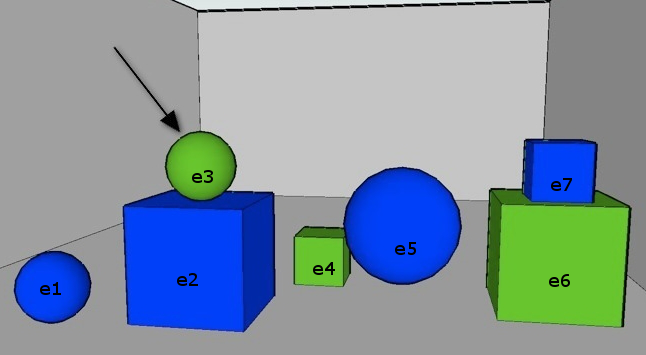
\includegraphics[width=0.5\textwidth]{images/3b.png}
\caption{Contexto de ejemplo}\label{GRE3D7-stimulus-cap2}
%\end{minipage}
\end{center}
\end{figure}

%\textcolor{blue}{hice mas grande la figura porque no se leian, como la pase a espaniol y se me fue al pie, no se porque}
%\hspace*{-0.35cm}
\begin{figure}[ht]
\begin{center}
%\begin{minipage}[b]{0.5\linewidth}
%\centering
\begin{tikzpicture}
  [
    n/.style={circle,fill,draw,inner sep=3pt,node distance=2.6cm},
    aArrow/.style={->, >=stealth, semithick, shorten <= 2pt, shorten >= 2pt},
  ]
 \node[n,label=below:{
    \relsize{-1}$\begin{array}{c}
      \nLeft\\[-2pt]
      \nSmall\\[-2pt] 
      \nBlue \\[-2pt] 
      \nBall\end{array}$}] (a) {$e_1$};

 \node[n,label=below:{
    \relsize{-1}$\begin{array}{c}
      \nLeft\\[-2pt]
      \nBig\\[-2pt] 
      \nBlue\\[-2pt] 
      \nCube\end{array}$}, right of=a] (b) {$e_2$};

 \node[n,label=above:{
    \relsize{-1}$\begin{array}{c}
      \nTop\\[-2pt]
      \nLeft\\[-2pt]
      \nSmall\\[-2pt] 
      \nGreen\\[-2pt] 
      \nBall\end{array}$}, above of=b] (c) {$e_3$};

 \node[n,label=below:{
    \relsize{-1}$\begin{array}{c}
      \nSmall\\[-2pt] 
      \nGreen\\[-2pt] 
      \nCube\end{array}$}, right of=b] (d) {$e_4$};

 \node[n,label=below:{
    \relsize{-1}$\begin{array}{c}
      \nBig\\[-2pt] 
      \nBlue\\[-2pt] 
      \nBall\end{array}$}, right of=d] (e) {$e_5$};

 \node[n,label=below:{
    \relsize{-1}$\begin{array}{c}
      \nBig\\[-2pt] 
      \nGreen\\[-2pt] 
      \nCube\end{array}$}, right of=e] (f) {$e_6$};

 \node[n,label=above:{
    \relsize{-1}$\begin{array}{c}
      \nTop\\[-2pt]
      \nSmall\\[-2pt] 
      \nBlue\\[-2pt] 
      \nCube\end{array}$}, above of=f] (g) {$e_7$};

 \draw [aArrow,bend right=90] (b) to node[auto,swap]{\relsize{-1}$\nBelow$} (c);
 \draw [aArrow,bend right=90] (c) to node[auto,swap]{\relsize{-1}$\nOntop$} (b);

 \draw [aArrow,bend right=70] (d) to node[auto,swap]{\relsize{-1}$\nLeftof$} (e);
 \draw [aArrow,bend right=70] (e) to node[auto,swap]{\relsize{-1}$\nRightof$} (d);

 \draw [aArrow,bend right=90] (f) to node[auto,swap]{\relsize{-1}$\nBelow$} (g);
 \draw [aArrow,bend right=90] (g) to node[auto,swap]{\relsize{-1}$\nOntop$} (f);

 \draw[dotted] (-.6,-2.2) rectangle (12.5,5.3);

 \end{tikzpicture}
\caption{Modelo relacional del Contexto \ref{GRE3D7-stimulus-cap2}}
\label{GRE3D7-stimulus-graph}
%\end{minipage}
\end{center}
\end{figure}

Algoritmos de refinamiento para GER se basan en la siguiente idea b\'asica:
dada una escena $S$, los objetos que aparecen en $S$ son sucesivamente
clasificados de acuerdo con sus propiedades en clases m\'as y m\'as finas. 
Una descripci\'on (en alg\'un lenguaje formal de $\mathcal{L}$) de cada
clase se calcula cada vez que una clase es refinada. El procedimiento siempre
se detiene cuando el conjunto de clases se estabiliza, es decir, no se puede hacer m\'as refinamiento
con la informaci\'on disponible en la escena \footnote{Por supuesto, si s\'olo estamos interesados en una expresi\'on referencial de un objeto dado, se puede detener el procedimiento en cuanto el objetivo es el
   \'unico elemento de alguna de las clases.}

Si el elemento target est\'a en
una clase singleton, entonces la descripci\'on formal de esa clase es un
expresi\'on referencial; de lo contrario el target no puede ser un\'{i}vocamente
descripto (en $\mathcal{L}$).

Est\'a claro que una escena puede ser codificada en diferentes formas como un
modelo relacional (por ejemplo, en \ref{GRE3D7-stimulus-cap2}, podr\'{i}amos argumentar que
$e_1$ es tambi\'en \emph{leftof} $e_2$, pero no lo consideramos porque no se estan 
tocando en la imagen). El algoritmo asume que estas cuestiones se han resuelto y que el modelo codifica una representaci\'on adecuada de la escena que
queremos describir. Por otra parte, vamos a suponer que todas las relaciones son
\emph{binarias}. No vamos a considerar las relaciones de aridad mayor que
dos (relaciones de mayor aridad pueden codificarse como relaciones binarias v\'{i}a
reificaci\'on, si es necesario).

%On termination, the algorithm computes what are called the
%$\mathcal{L}$-similarity classes of the input model $\gM$.
%Intuitively, the referring expression ``\textsf{ball}'' and ``\textsf{cube}''  are more specific and then contain more information than $\top$.


Tras la resoluci\'on, el algoritmo calcula lo que se llama la
$\mathcal{L}$ - clases de semejanza del modelo de entrada de $\gM$.\\

%There is many $\mathcal{L}$, we will name $\alc$ y $\el$

%ACA VOY A PONER gramatica para generar... ALC y EL no quedaria bien aca, hay que ver lo agregamos antes o no hace falta
%In what follows, we use formulas of the $\el$ description logic
%language
En lo que sigue, se utilizan f\'ormulas de la descripci\'on de la l\'ogica $\el$
~\cite{baad:desc03} para describir las clases de refinamiendo
\footnote{N\'otese, sin embargo, que el lenguaje formal particular usado es
   independiente del algoritmo principal, y diferentes funciones
  add$_{\mathcal{L}}$($\varphi$,\RE) se pueden utilizar dependiendo
   de la l\'ogica en cuesti\'on.}. como se discuti\'o 
en~\cite{arec2:2008:Areces}, 
este lenguaje es adecuado para describir
RE conjuntivas y relacionales, que son lo que encontramos en los corpus.

  La entrada al algoritmo ser\'a un modelo $\mathcal{M} =
 \tup{\Delta, \interp{\cdot}}$, donde $\Delta$ es el dominio no vac\'io de objetos de la imagen,
 $\interp{\cdot}$ es una funci\'on de interpretaci\'on que asigna a todas las propiedades de la escena su extensi\'on.
 Por ejemplo, la escena mostrada en la Figura~\ref{GRE3D7-stimulus-cap2} podr\'ia ser representada por el modelo
 $\gM=\tup{\Delta,\interp{\cdot}}$ mostrado en la 
 Figura~\ref{GRE3D7-stimulus-graph}; donde+- $\Delta =
 \{e_1,\ldots,e_7\}$, e $\interp{\textsf{red}}$ is $\{e_2, e_4, e_5,
 e_7\}$.

Se llama extensi\'on de una f\'ormula al conjunto de objetos que la hacen v\'alida.

$\top$ es una f\'ormula que representa la descripci\'on m\'as general, cuya
interpretaci\'on incluye todos los elementos del modelo. Se podr\'ia realizar
como la ER con el sustantivo
``\textsf{cosa}''. Decimos que una f\'ormula es
\emph{subsumida} por otras f\'ormulas, cuando su extensi\'on puede ser cubierta por la
union de las extensiones de las otras f\'ormulas. Por ejemplo, en la
Figura~\ref{GRE3D7-stimulus-cap2}, $\top$ es subsumida por ``\textsf{esfera}'' y
``\textsf{cubo}'', porque $\interp{\top}$ = $\interp{\textsf{esfera}}
\cup \interp{\textsf{cube}}$.
%= $\{e_2, e_4, e_6, e_7\}$, it is $\{e_1, e_2, e_3, e_4, e_5, e_6, e_7\}$ = $\{e_1, e_3, e_5\} \cup \{e_2, e_4, e_6, e_7\}$. 
Intuitivamente la f\'ormula ``\textsf{cubo}'' o ``\textsf{esfera}'' tienen m\'as informaci\'on que $\top$, para cada elemento de $\top$, hay una f\'ormula que d\'a m\'as informaci\'on, digamos ``\textsf{cubo}'' es m\'as informativa que ``\textsf{cosa}''.\\

%In the following we will explain an example of execusion of the
%algorithm shown in Figure
%A continuaci\'on vamos a explicar un ejemplo de ejecusi\'on del
%algoritmo mostrado en la Figura~\ref{algoritmoOriginal} considerando la l\'ogica 
%$\el$ como language. Este algoritmo fue presentado en
%~\cite{arec2:2008:Areces}.
%
%\begin{figure}[h!]
%\begin{center}
%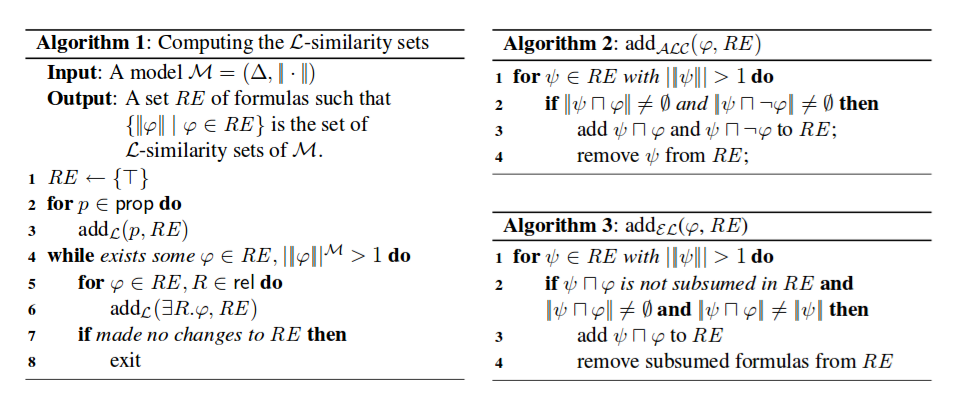
\includegraphics[width=\textwidth]{images/algoritmoOriginal.png}
%\end{center}
%\vspace*{-2em}
%\caption{Algoritmo para GER con l\'ogicas de descripci\'on}
%\label{algoritmoOriginal}
%\end{figure}

%\subsection{Ejemplo de ejecuci\'on}
%
%
%
%\textcolor{blue}{no se si poner aca un ejemplo, si poner el texto y las im\'agenes en otro apendice... o ponerlas mas chiquitas en varias columnas, asi queda feo}\\
%Vamos a ejecutar el algoritmo para la Figura~\ref{GRE3D7-stimulus-cap2},
%el algoritmo comienza con una lista fija de propiedades y relaciones, supongamos que
%esas listas son las siguientes:
%
%propiedades ordenadas (prop): \textsf{ball}, \textsf{cube}, \textsf{red}, \textsf{yellow}, \textsf{small}, \textsf{large}.\\
%relaciones ordenadas (rel): \textsf{leftof}, \textsf{rightof}, \textsf{ontopof}, \textsf{bellowof}.
%
%%\begin{figure}
%%\begin{center}	
%%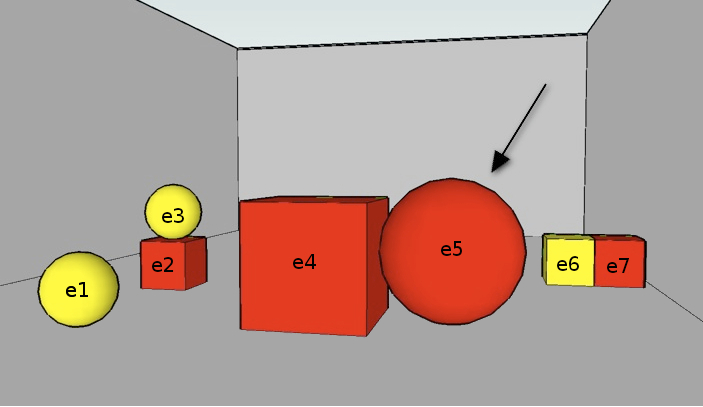
\includegraphics[width=.5\textwidth]{images/22.jpg}
%%\end{center}
%%\vspace*{-1.5em}
%%\caption{Escena 3D de figuras geom\'etricas}\label{figure22}
%%\end{figure}
%
%%\begin{figure}
%%\begin{minipage}[b]{0.6\linewidth}
%%\centering
%%\begin{tikzpicture}
%%  [
%%    n/.style={circle,fill,draw,inner sep=3pt,node distance=1.4cm},
%%    aArrow/.style={->, >=stealth, semithick, shorten <= 2pt, shorten >= 2pt},
%%  ]
%% \node[n,label=above:$e_1$,label=below:{
%%    \relsize{-1}$\begin{array}{c}
%%      \nLeft\\[-2pt]
%%      \nSmall\\[-2pt] 
%%      \nYellow \\[-2pt] 
%%      \nBall\end{array}$}] (a) {};
%
%% \node[n,label=above:$e_2$,label=below:{
%%    \relsize{-1}$\begin{array}{c}
%%      \nLeft\\[-2pt]
%%      \nSmall\\[-2pt] 
%%      \nRed\\[-2pt] 
%%      \nCube\end{array}$}, right of=a] (b) {};
%
%% \node[n,label=below:$e_3$,label=above:{
%%    \relsize{-1}$\begin{array}{c}
%%      \nTop\\[-2pt]
%%      \nLeft\\[-2pt]
%%      \nSmall\\[-2pt] 
%%      \nYellow\\[-2pt] 
%%      \nBall\end{array}$}, above of=b] (c) {};
%
%% \node[n,label=above:$e_4$,label=below:{
%%    \relsize{-1}$\begin{array}{c}
%%      \nBig\\[-2pt] 
%%      \nRed\\[-2pt] 
%%      \nCube\end{array}$}, right of=b] (d) {};
%
%% \node[n,label=above:$e_5$,label=below:{
%%    \relsize{-1}$\begin{array}{c}
%%      \nBig\\[-2pt] 
%%      \nRed\\[-2pt] 
%%      \nBall\end{array}$}, right of=d] (e) {};
%
%% \node[n,label=above:$e_6$,label=below:{
%%    \relsize{-1}$\begin{array}{c}
%%      \nSmall\\[-2pt] 
%%      \nYellow\\[-2pt] 
%%      \nCube\end{array}$}, right of=e] (f) {};
%
%% \node[n,label=above:$e_7$,label=below:{
%%    \relsize{-1}$\begin{array}{c}
%%      \nSmall\\[-2pt] 
%%      \nRed\\[-2pt] 
%%      \nCube\end{array}$}, right of=f] (g) {};
%
%% \draw [aArrow,bend right=90] (b) to node[auto,swap]{\relsize{-1}$\nBelow$} (c);
%% \draw [aArrow,bend right=90] (c) to node[auto,swap]{\relsize{-1}$\nOntop$} (b);
%
%% \draw [aArrow,bend right=30] (d) to node[auto,swap]{\relsize{-1}$\nLeftof$} (e);
%% \draw [aArrow,bend right=30] (e) to node[auto,swap]{\relsize{-1}$\nRightof$} (d);
%
%% \draw [aArrow,bend right=30] (f) to node[auto,swap]{\relsize{-1}$\nLeftof$} (g);
%% \draw [aArrow,bend right=30] (g) to node[auto,swap]{\relsize{-1}$\nRightof$} (f);
%
%% \draw[dotted] (-.4,-1.7) rectangle (7.5,3.3);
%
%% \end{tikzpicture}
%%\caption{La escena como modelo relacional}\label{GRE3D7-stimulus-graph}
%%\end{minipage}
%%\end{figure}
%
%
%El algoritmo siempre termina, y devuelve ER un conjunto de f\'ormulas que describe cada elemento en el dominio (si existe esa f\'ormula). \\
%
%En el comienzo ER=$\{\top\}$ y $\interp{\top}$ = $\{e_1, e_2, e_3, e_4, e_5, e_6, e_7\}$ como se puede ver en la Figura~\ref{fig-modelo}.\\
%
%ACA
%\begin{figure}[ht]
%\begin{minipage}[b]{0.45\linewidth}
%\centering
%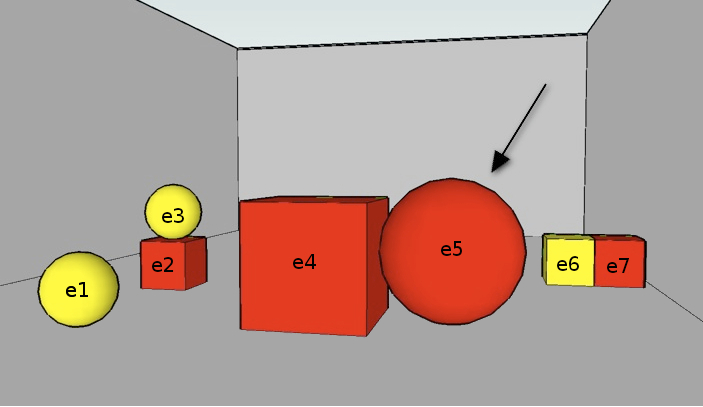
\includegraphics[width=\textwidth]{images/22.jpg}
%\vspace*{1cm}
%%\caption{Input scene}
%\label{GRE3D7-stimulus-22}
%\end{minipage}
%%\hspace*{-0.35cm}
%\begin{minipage}[b]{0.6\linewidth}
%\centering
%%\begin{figure}[ht]
%%\begin{center}
%\frame{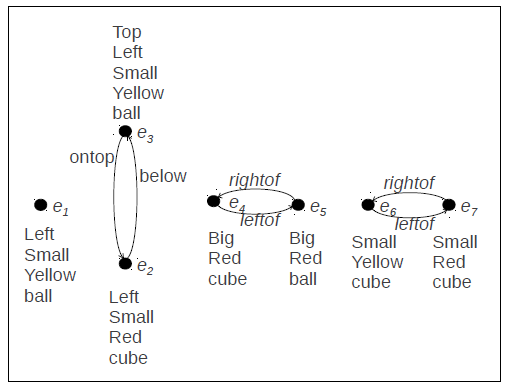
\includegraphics[width=8cm]{images/modelo.png}}\\[0pt]
%\caption{Modelo de la Figura \ref{GRE3D7-stimulus-22}}
%\label{fig-modelo}
%\end{minipage}
%\end{figure}
%El primer bucle del algoritmo es en las propiedades. Para cada propiedad hace add$_\el$ ($\varphi$, RE), las propiedades at\'omicas se muestran en la Figura~\ref{fig-modelo2}.
%
%\begin{figure}[ht]
%\begin{center}
%\frame{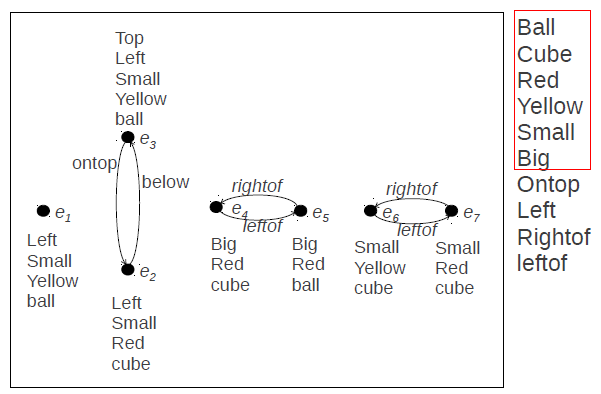
\includegraphics[width=8cm]{images/modelo2.png}}\\[0pt]
%\caption{Propiedades proposicionales en cuadro rojo, las del primer ciclo del algoritmo}
%\label{fig-modelo2}
%\end{center}
%\end{figure}
%
%La f\'ormula $\varphi$ se a\~nadir\'a a ER si su interpretaci\'on tiene al menos un elemento, a continuaci\'on, para cada f\'ormula
 %$\psi$ en ER la conjunci\'on
%$\varphi  \wedge \psi$ no necesita estar subsumida in ER, la $\interp{\varphi \cup \psi}$ no tiene que ser vac\'io, y su interpretaci\'on tiene que ser distinta de $\interp{\psi}$. Luego las f\'ormulas subsumidas se borran.
%
%La primer propiedad es \textsf{ball}, ER = \{$\top$, \textsf{ball}\}, se ven los elementos de ``ball'' en un recuadro en la Figura~\ref{fig-modelo3}.
%
%\begin{figure}[ht]
%\begin{center}
%\frame{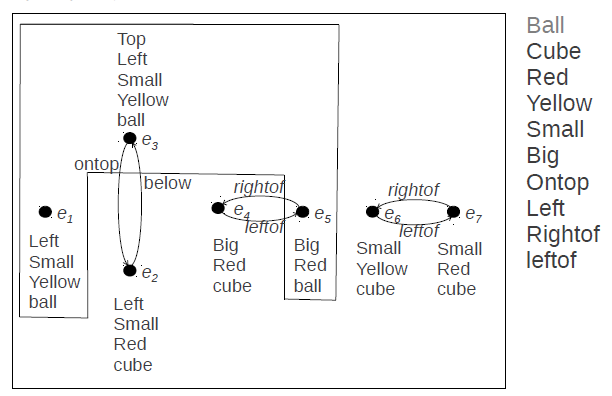
\includegraphics[width=8cm]{images/modelo3.png}}\\[0pt]
%\caption{El cuadro indica cuales son ``ball''}
%\label{fig-modelo3}
%\end{center}
%\end{figure}
%
%La siguiente propiedad es \textsf{cube}, ER = \{$\top$, \textsf{ball}, \textsf{cube}\}, pero ahora la $\interp{\textsf{ball}}$ = $\{e_1, e_3, e_5\}$, $\interp{\textsf{cube}}$ = $\{e_2, e_4, e_6, e_7\}$, quedando las particiones como se muestra en la Figura~\ref{fig-modelo4}
%\begin{figure}[ht]
%\begin{center}
%\frame{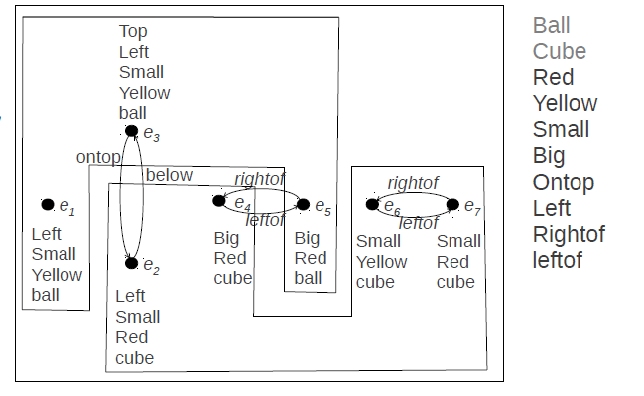
\includegraphics[width=8cm]{images/modelo4.png}}\\[0pt]
%\caption{Cuadros indicando ``ball'' y ``cube''}
%\label{fig-modelo4}
%\end{center}
%\end{figure}
%Ahora podemos borrar $\top$, porque es subsumida (esta cubierta por) las otras dos f\'ormulas. La siguiente propiedad es  \textsf{red}, $\interp{\textsf{red}}$ es: $\{e_2, e_4, e_5, e_7\}$, haciendo la intersecci\'on con la $\interp{.}$ de cada f\'ormula en ER obtenemos, $\{e_5\}$ y $\{e_2, e_4, e_7\}$, ER = $\{\textsf{ball}, \textsf{cube}, \textsf{ball} \wedge \textsf{red}, \textsf{cube} \wedge \textsf{red}\}$, las particiones actuales se pueden ver en la Figura~\ref{fig-modelo9}.
%\begin{figure}[ht]
%\begin{center}
%\frame{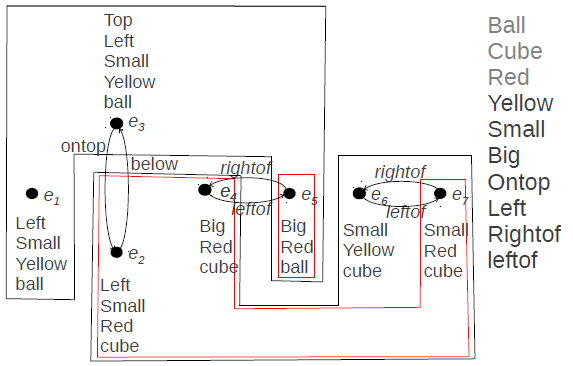
\includegraphics[width=8cm]{images/modelo9.png}}\\[0pt]
%\caption{Cuadros indicando ``ball'', ``cube'' y ``red''}
%\label{fig-modelo9}
%\end{center}
%\end{figure}
%
%Siguiendo con \textsf{yellow}, tenemos, $\interp{\textsf{yellow}}$ = $\{e_1, e_3, e_6\}$ y obtenemos ER = $\{\textsf{ball} \wedge \textsf{yellow}, \textsf{cube} \wedge \textsf{yellow}, \textsf{ball} \wedge \textsf{red}, \textsf{cube} \wedge \textsf{red}\}$. 
%Note que aqu\'i ya borramos la f\'ormula \textsf{ball} porque estaba subsumida, y la f\'ormula \textsf{cube} tambi\'en. Se muestran particiones en Figura~\ref{fig-modelo10}.
%
%\begin{figure}[ht]
%\begin{center}
%\frame{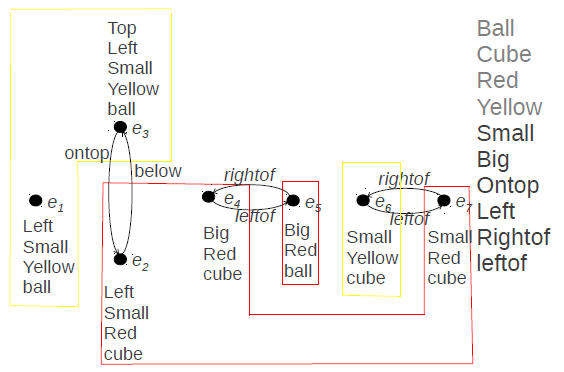
\includegraphics[width=8cm]{images/modelo10.png}}\\[0pt]
%\caption{Cuadros indicando ``ball'', ``cube'', ``red'' y ``yellow''}
%\label{fig-modelo10}
%\end{center}
%\end{figure}
%
%Haciendo lo mismo con \textsf{small} tenemos ER = $\{\textsf{ball} \wedge \textsf{yellow} \wedge \textsf{small}, \textsf{cube} \wedge \textsf{yellow} \wedge \textsf{small}, \textsf{ball} \wedge \textsf{red}, \textsf{cube} \wedge \textsf{red}, \textsf{cube} \wedge \textsf{red} \wedge \textsf{small}\}$, como se puede ver en Figura~\ref{fig-modelo11}.
%\begin{figure}[ht]
%\begin{center}
%\frame{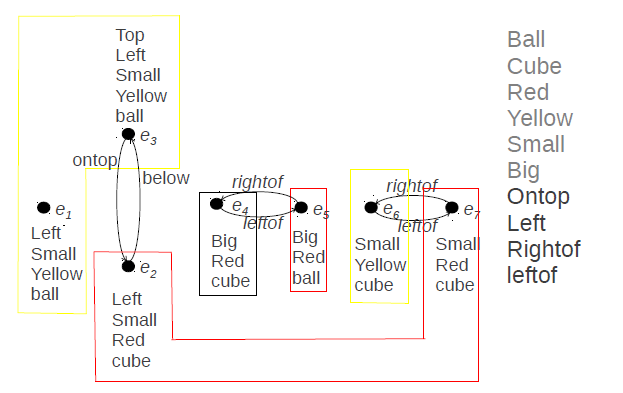
\includegraphics[width=8cm]{images/modelo11.png}}\\[0pt]
%\caption{Cuadros indicando ``ball'', ``cube'', ``red'', ``yellow'', ``small'' y ``large''}
%\label{fig-modelo11}
%\end{center}
%\end{figure}
%
%La siguiente propiedad es \textsf{large} as\'i, tenemos ER = $\{\textsf{ball} \wedge \textsf{yellow} \wedge \textsf{small}, \textsf{cube} \wedge \textsf{yellow} \wedge \textsf{small}, \textsf{ball} \wedge \textsf{red}, \textsf{cube} \wedge \textsf{red} \wedge \textsf{large}, \textsf{cube} \wedge \textsf{red} \wedge \textsf{small}\}$. Aqu\'i no podemos agregar \textsf{large} a la f\'ormula $\textsf{red} \wedge \textsf{cube}$ porque su interpretaci\'on tiene un solo elemento, y la condici\'on dice que es necesario tener m\'as de uno.
%
%Hasta ahora ER = $\{\textsf{ball} \wedge \textsf{yellow} \wedge \textsf{small}, \textsf{cube} \wedge \textsf{yellow} \wedge \textsf{small}, \textsf{ball} \wedge \textsf{red}, \textsf{cube} \wedge \textsf{red} \wedge \textsf{large}, \textsf{cube} \wedge \textsf{red} \wedge \textsf{small}\}$ 
%y tenemos las siguientes extensiones: $\{e_1, e_3\}, \{e_6\}, \{e_5\}, \{e_4\}, \{e_2, e_7\}$ respectivamente. 
%Hay dos f\'ormulas que a\'un pueden ser refinadas, $\textsf{ball} \wedge \textsf{yellow} \wedge \textsf{small}$ y $\textsf{cube} \wedge \textsf{red} \wedge \textsf{small}$ 
%debido a que tienen m\'as de un elemento cada una, por lo que entran en el ciclo, while del algoritmo 1, en la l\'inea 4. Ahora es el turno de las relaciones, la primera de ellas es \textsf{leftof}, para cada f\'ormula $\varphi$ en ER trataremos de hacer add$_\el$ ($\exists \textsf{leftof}.\varphi$, RE). Notar que $\psi$ solo puede ser $\textsf{ball} \wedge \textsf{yellow} \wedge \textsf{small}$ o $\textsf{cube} \wedge \textsf{red} \wedge \textsf{small}$ porque esos son los que su interpretaci\'on tiene m\'as de un elemento. 
%\begin{figure}[ht]
%\begin{center}
%\frame{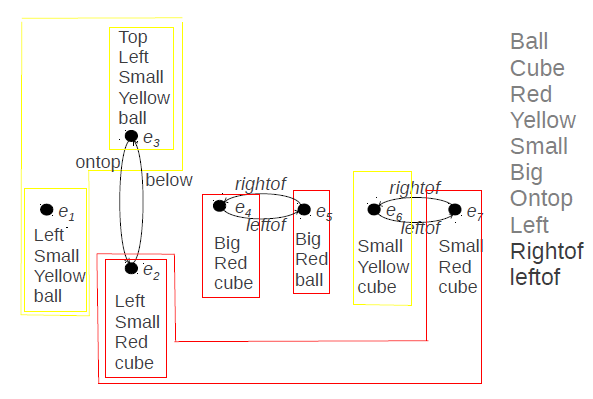
\includegraphics[width=8cm]{images/modelo15.png}}\\[0pt]
%\caption{Cuadros indicando ``ball'', ``cube'', ``red'', ``yellow''...}
%\label{fig-modelo15}
%\end{center}
%\end{figure}
%
%
%No hay
%%because those are the ones that its interpretation have more than one element. There is not 
%$\varphi$ y $\psi$ que puedan ser aplicadas. Continuando con \textsf{rightof} agregamos $\textsf{cube} \wedge \textsf{yellow} \wedge \textsf{small} \wedge \exists \textsf{rightof}. \textsf{cube} \wedge \textsf{red} \wedge \textsf{small}$, y asi con \textsf{topof} agregamos $\textsf{small} \wedge \textsf{red} \wedge \textsf{cube} \wedge \exists \textsf{ontop}. \textsf{small} \wedge \textsf{yellow} \wedge \textsf{ball}$ y el algoritmo termina con ER = $\{\textsf{ball} \wedge \textsf{yellow} \wedge \textsf{small}, \textsf{cube} \wedge \textsf{yellow} \wedge \textsf{small}, \textsf{ball} \wedge \textsf{red}, \textsf{cube} \wedge \textsf{red} \wedge \textsf{large}, \textsf{cube} \wedge \textsf{red} \wedge \textsf{small}, \textsf{cube} \wedge \textsf{yellow} \wedge \textsf{small} \wedge \exists \textsf{rightof}. \textsf{cube} \wedge \textsf{red} \wedge \textsf{small}, \textsf{small} \wedge \textsf{red} \wedge \textsf{cube} \wedge \exists \textsf{ontop}. \textsf{small} \wedge \textsf{yellow} \wedge \textsf{ball}\}$, 
%aqu\'i todos los elementos est\'an en una clase singleton y no se puede hacer ning\'un refinamiento m\'as. 
%%can be applied to $cube \wedge red \wedge small$ but there is no formula which interpretation has more than one element to be apply with this one. The same happen for the other relations, so the algorithm ends.
%%its interpretation is $\{e_7\}$ with $\psi$ is $cube \wedge yellow \wedge small$, the others combinations can't be apply because they don't do true the preconditions. The following relation is rightof, 
%
%%leftof, rightof, ontopof, bellowof
%
%%At this point we already have the target in a singleton set. So the formula for it is ``red and ball'', and also for s6 which formula is ``yellow cube''.\\
%%As we show this algorithm depends of the order of properties and relations.\\
%\begin{figure}[ht]
%\begin{center}
%\frame{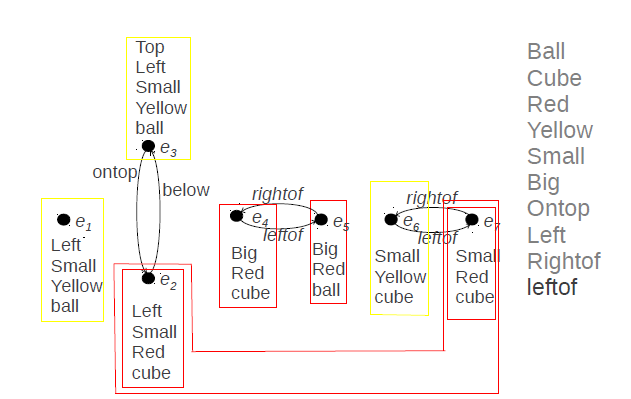
\includegraphics[width=8cm]{images/modelo16.png}}\\[0pt]
%\caption{Cuadros indicando ``ball'', ``cube'', ``red'', ``yellow''...}
%\label{fig-modelo16}
%\end{center}
%\end{figure}
%
%\begin{figure}[ht]
%\begin{center}
%\frame{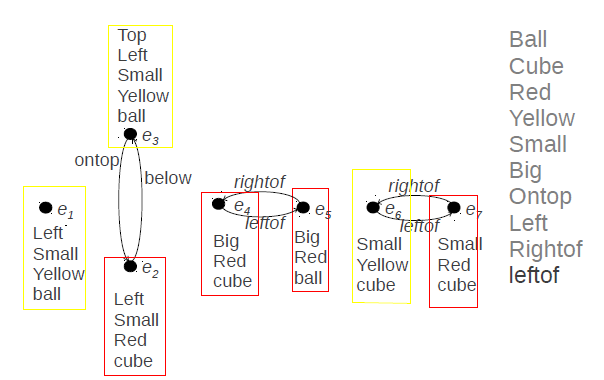
\includegraphics[width=8cm]{images/modelo17.png}}\\[0pt]
%\caption{Cuadros indicando ``ball'', ``cube'', ``red'', ``yellow''...}
%\label{fig-modelo17}
%\end{center}
%\end{figure}
%
%Las expresiones referenciales encontradas son:\\
%
%$\textsf{ball} \wedge \textsf{yellow} \wedge \textsf{small}$ representa $e_1$ \\
%$\textsf{cube} \wedge \textsf{yellow} \wedge \textsf{small}$ representa $e_6$ \\
%$\textsf{ball} \wedge \textsf{red}$ representa $e_5$ \\
%$\textsf{cube} \wedge \textsf{red} \wedge \textsf{large}$ representa $e_4$ \\
%$\textsf{cube} \wedge \textsf{red} \wedge \textsf{small}$ representa $\{e_2,e_7\}$  \\
%$\textsf{cube} \wedge \textsf{yellow} \wedge \textsf{small} \wedge \exists \textsf{rightof}. \textsf{cube} \wedge \textsf{red} \wedge \textsf{small}$ representa $e_6$ \\
%$\textsf{small} \wedge \textsf{red} \wedge \textsf{cube} \wedge \exists \textsf{ontop}. \textsf{small} \wedge \textsf{yellow} \wedge \textsf{ball}$ representa $e_2$ \\
%



%\section{Aproximaciones emp\'iricas a la soluci\'on de GER}
%\label{sec:trabajos_empiricos}
%
%
%
%
%\subsection{Trabajos emp\'iricos en el \'area}
%\label{sec:trab_emp}

%http://link.springer.com/chapter/10.1007/978-3-642-15573-4_9
%http://www.jetteviethen.net/papers/DaleViethen2010chapter.pdf


%%ROMI---
%\newcommand{\instFun}[2]{\texttt{#1}\ensuremath{_{#2}}\xspace}

%\section{GRE via Building Simulated Models}\label{sec:krahmer}

Krahmer~et~al.~\cite{Krahmer2003} introducen un algoritmo para computar la determinaci\'on de
contenido basado en computaci\'on de \emph{isomorfismos de subgrafos}.

Est\'a fuertemente regulado por las funciones de costo y por lo tanto es apto para poner en pr\'actica
diferentes preferencias. De hecho, muestran que el uso de las funciones de costos adecuadas
puede simular la mayor\'ia de las propuestas anteriores. Su algoritmo toma como entrada
un grafo dirigido etiquetado $G$ y un nodo $e$ y devuelve, si es posible,
un subgrafo conectado $H$  de $G$, que contiene $e$ y suficiente informaci\'on conectada para
distinguir a $e$ de los otros nodos.

Ahora identificaremos la noci\'on de expresividad subyacente y como se puede extender.
Para mantener la terminolog\'ia de~\cite{Krahmer2003}, en lo que sigue
podemos hablar alternativamente de \emph{grafos etiquetados} en lugar de modelos relacionales.
El lector debe observar que son esencialmente el mismo objeto matem\'atico, pero codifican las propiedades proposicionales utilizando
loops de relaciones binarias (por ejemplo, escriben $\nDog(e,e)$ en vez de $\nDog(e)$).

The main ideas of their algorithm can be
intuitively summarized as follows.
Given two labeled graphs $H$ and $G$, and vertices $v$ of $H$
and $w$ of $G$, we say that the pair $(v,H)$ {\em refers}
to the pair $(w,G)$ iff $H$ is connected and $H$ can be ``placed
over'' $G$ in such a way that: 1) $v$ is placed over $w$; 2) each
node of $H$ is placed over a node of $G$ with at least the same
unary predicates (but perhaps more); and 3) each edge from $H$ is
placed over an edge with the same label. Furthermore, $(v,H)$ {\em
uniquely refers} to $(w,G)$ if $(v,H)$ refers to $(w,G)$ and there
is no vertex $w'\not=w$ in $G$ such that $(v,H)$ refers to $(w',G)$.
The formal notion of a labeled graph being ``placed over'' another
one is that of {\em subgraph isomorphism}:
$H=\tup{\Delta_H,\interp{\cdot}_H}$ can be placed over
$G$ iff there is a labeled subgraph (i.e., a graph obtained from
$G$ by possibly deleting certain nodes, edges, and propositions from some nodes)
$G'=\tup{\Delta_{G'},\interp{\cdot}_{G'}}$ of $G$ such that $H$ is {\em
isomorphic} to $G'$, which means that there is a
bijection


La idea principal de su algoritmo puede resumirse intuitivamente como sigue.
Dados dos grafos etiquetados $H$ y $G$, y los v\'ertices  $v$ de $H$
y $w$ de $G$, decimos que el par $(v, H)$ {\em refiere}
al par $(w, G)$ si y s\'olo si $H$ est\'a conectado y $H$ puede ser colocado ``
sobre'' $G$ de tal manera que: 1) $v$ se coloca sobre $w$; 2) cada
nodo de $H$ se coloca sobre un nodo de $G$ con al menos el mismo
predicados unarios (pero tal vez m\'as); y 3) de cada arista de $H$ es
colocado sobre una arista con la misma etiqueta. Por otra parte, $(v, H)$ {\em
se refiere \'unicamente a} $(w, G)$ si $(v, H)$ se refiere a $(w, G)$ y no hay
v\'ertice $w'\not=w$ in $G$ tal que $(v, H)$ se refiere a $(w', G)$.
La noci\'on formal de un grafo ``colocado sobre'' otro es el de {\em subgrafo isomorfo}:
$H=\tup{\Delta_H,\interp{\cdot}_H}$ se puede colocar sobre
$G$ si y s\'olo si existe un subgrafo marcado (es decir, un grafo obtenido a partir de
$G$ posiblemente por la eliminaci\'on de ciertos nodos, bordes y proposiciones de algunos nodos)
$G'=\tup{\Delta_{G'},\interp{\cdot}_{G'}}$ de $G$ tal que $H$ es {\em
isomorfo} ​​para $G'$, lo que significa que hay una biyecci\'on

 $f:\Delta_{H}\to\Delta_{G'}$ such that for all vertices
$u,v\in \Delta_H$, $u\in\interp{p}_{H}$ iff $f(u)\in\interp{p}_{G'}$
and $(u,v)\in\interp{r}_{H}$ iff $(f(u),f(v))\in\interp{r}_{G'}$.
%
\begin{figure}
\centering
\begin{tabular}{c@{\hspace{1.0cm}}c@{\hspace{1.0cm}}c@{\hspace{1.0cm}}c}
\begin{picture}(22,50)
\put(0,0){\begin{tikzpicture}
  [
    n/.style={circle,fill,draw,inner sep=1.5pt,node distance=1.5cm},
    aSniffing/.style={->, >=stealth, semithick, shorten <= 3pt, shorten >= 3pt},
  ]
 \node[n,label=above:$v$,label=below:{\relsize{-1}$\begin{array}{c}\nDog\\\ \end{array}$}] (a) {};
 \end{tikzpicture}}
 \end{picture}
&
\begin{picture}(55,50)
\put(0,0){\begin{tikzpicture}
  [
    n/.style={circle,fill,draw,inner sep=1.5pt,node distance=1.5cm},
    aSniffing/.style={->, >=stealth, semithick, shorten <= 3pt, shorten >= 3pt},
  ]
 \node[n,label=above:,label=below:{\relsize{-1}$\begin{array}{c}\ \end{array}$}] (a) {};

 \node[n,label=above:$v$,label=below:{\relsize{-1}$\begin{array}{c}\nDog\\\ \end{array}$}, right of=a] (b) {};

 \draw [aSniffing,bend right=40] (b) to node[auto,swap]{\relsize{-1}$\aSniffing$} (a);

 \end{tikzpicture}}
 \end{picture}
&
\begin{picture}(70,50) \put(0,0){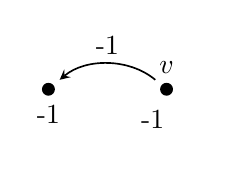
\begin{tikzpicture}
  [
    n/.style={circle,fill,draw,inner sep=1.5pt,node distance=1.5cm},
    aSniffing/.style={->, >=stealth, semithick, shorten <= 3pt, shorten >= 3pt},
  ]
 \node[n,label=above:,label=below:{\relsize{-1}$\begin{array}{c}\nDog\end{array}$}] (a) {};

 \node[n,label=above:$v$,label=below:{\relsize{-1}$\begin{array}{c}\nDog\\ \aSmall \end{array}$}, right of=a] (b) {};

 \draw [aSniffing,bend right=40] (b) to node[auto,swap]{\relsize{-1}$\aSniffing$} (a);

 \end{tikzpicture}}
 \end{picture}
&
\begin{picture}(77,50)
\put(0,0){\begin{tikzpicture}
  [
    n/.style={circle,fill,draw,inner sep=1.5pt,node distance=1.5cm},
    aSniffing/.style={->, >=stealth, semithick, shorten <= 3pt, shorten >= 3pt},
  ]
 \node[n,label=above:$v$,label=below:{\relsize{-1}$\begin{array}{c}\nDog\end{array}$}, right of=a] (b) {};
%
 \node[n,label=above:,label=below:{\relsize{-1}$\begin{array}{c}\nCat\\ \aSmall\end{array}$}, right of=b] (c) {};
%
 \draw [aSniffing,bend right=40] (c) to node[auto,swap]{\relsize{-1}$\aSniffing$} (b);
 \end{tikzpicture}}
 \end{picture}
% %
% \begin{picture}(77,50)
% \put(0,0){\begin{tikzpicture}
%   [
%     n/.style={circle,fill,draw,inner sep=1.5pt,node distance=1.5cm},
%     aSniffing/.style={->, >=stealth, semithick, shorten <= 3pt, shorten >= 3pt},
%   ]
%  \node[n,label=above:,label=below:{\relsize{-1}$\begin{array}{c}\end{array}$}] (a) {};
%
%  \node[n,label=above:$v$,label=below:{\relsize{-1}$\begin{array}{c}\end{array}$}, right of=a] (b) {};
%
%  \draw [aSniffing,loop left] (a) to node[above,xshift=-5pt]{\relsize{-1}$\aSniffing$} (a);
%
%  \draw [aSniffing,bend right=40] (b) to node[auto,swap]{\relsize{-1}$\aSniffing$} (a);
%  \end{tikzpicture}}
%  \end{picture}
\vspace{-.2cm}\ \\
(i)&(ii)&(iii)&(iv)
\end{tabular}
 \caption{Algunos subgrafos conectados $(v,H)$ de la escena $\+S$ de la Figura~\ref{fig:cat-dog-1}.\label{fig:subgraphs}}
 \end{figure}

As an example, consider the relational model depicted in
Figure~\ref{fig:cat-dog-1} as a labeled graph $G$, and let us
discuss the pairs of nodes and connected subgraphs $(v,H)$ shown in
Figure~\ref{fig:subgraphs}. Clearly, (i) refers to the pair $(w,G)$
for any node $w\in\{a,b,d\}$; (ii) refers to $(w,G)$ for
$w\in\{b,d\}$; and both (iii) and (iv) uniquely refer to $(b,G)$. Notice
that (i)--(iv) can be respectively realized as ``{\em a dog}'',
``{\em a dog that sniffs something}'', ``{\em a small dog that
sniffs a dog}'' (cf. $\gamma_1$ in Table~\ref{tab:gammas}) % and ``{\em
% something that
% sniffs something else that sniffs itself}''.
and ``{\em the dog that is sniffed by a small cat}'' (cf.~$\gamma_4$ in
Table~\ref{tab:gammas}).


Como ejemplo, consideremos el modelo relacional que se representa en la
La Figura~\ref{fig:cat-dog-1} como un grafo etiquetado $G$, y consideremos los pares de nodos conectados y subgrafos $(V, H)$ que se muestran en 
La Figura~\ref{fig:subgraphs}. Est\'a claro que (i) se refiere a la pareja $(w, G)$
para cualquier nodo $w\in\{a,b,d\}$; (ii) se refiere a $(w, G)$ para
$w\in\{b,d\}$; y ambos (iii) y (iv) se refieren \'unicamente a $(b, G)$. Notar
que (i) -- (iv) pueden realizarse, como  ``{\em a dog}'',
``{\em a dog that sniffs something}'', ``{\em a small dog that
sniffs a dog}'' respectivamente ($\gamma_1$ en la Tabla~\ref{tab:gammas}) y ``{\em the dog that is sniffed by a small cat}'' ($\gamma_4$ en
Table~\ref{tab:gammas}

% \fxnote{\tiny Reescribir los siguientes dos parrafos. Decir algo como, 'once
% more we'll try to remain as close as possible to the algorithms of the original
% article and we will then start by pointing out the differences with the algorithms
% we presented in the previous section'}

Es importante destacar que hay una diferencia sustancial
entre el algoritmo presentado en~\cite{Krahmer2003} y el que discutimos
en los apartados anteriores:
% First note that scenes are encoded in that article in a slightly
% different way: there, graphs have only labels on edges, and
% non-relational attributes such as \emph{type} or \emph{color} are
% represented by loops (e.g., $\aSmall(a,a)$). % \fxnote{\tiny Aca decia
% `While our presentation is, arguably, conceptually cleaner, it
% forces us to treat the atomic and relational cases separately'. No
% hablemos de `our presenation' respecto de la de la seccion anterior.
% O ninguna o las dos son `our presentation'. }
%

Mientras que la entrada es un grafo etiquetado $G$ y un nodo target $v$, la
salida es, en este caso (a diferencia de la definici\'on del problema de $\+L$-GER 
presentado anteriormente donde la salida es una {\em f\'ormula}), la de menor costo (con
respecto a algunos, la funci\'on de costo anteriormente especificada) 
{\em subgrafo} conectado $H$ de $G$, que se refiere \'unicamente a $(v, G)$ si hay
tales $H$ y $\bot$ en caso contrario.

No vamos a tratar con funciones de costo aqu\'i; es suficiente con saber
que una funci\'on de costo es una funci\'on mon\'otona que asigna a cada
subgrafo de un grafo de escena de un n\'umero no negativo que expresa la
bondad de un subgrafo. Por ejemplo en la Figura~\ref{fig:subgraphs}, uno
puede sintonizar la funci\'on de costo de modo que (iii) tenga menor costo que (iv), y por lo tanto
dar preferencia, a (iii) en vez de a (iv).

%By defining cost functions in
%different ways, \cite{Krahmer2003} shows that it is possible to mimic various algorithms for the
%generation of referring expressions known from the literature.

For reasons of space we will not introduce here the detailed algorithm proposed
in~\cite{Krahmer2003}. Roughly, it is a
straightforward branch and bound algorithm that systematically tries all
relevant subgraphs $H$ of $G$ by starting with the subgraph
containing only vertex $v$ and expanding it recursively by trying to
add edges from $G$ that are adjacent to the subgraph $H$ constructed
up to that point. In the terminology
of~\cite{Krahmer2003} a {\em distractor} is a node of $G$ different from
$v$ that is also referred by $H$.
The algorithm ensures that a subgraph uniquely refers to the
target $v$ when it has no distractors. Reached this point we
have a new candidate for the solution, but there can be other
cheaper solution so the search process continues until the
cheapest solution is detected. Cost functions are used to
guide the search process and to give preference to some solutions
over others.
% In the definition of~\cite{Krahmer2003}, $H$ is  such that every \emph{subgraph isomorphism}
% $f$ between $H$ and $G$ (i.e., every isomorphism between $H$
%  and a subgraph of $G$)
%  satisfies $f(u) = u$.
%
El sistema propuesto en~\cite{Krahmer2003} es una
versi\'on sencilla del algoritmo de cota que trata sistem\'aticamente todos los
subgrafos pertinentes $H$ de $G$ comenzando con el subgrafo
que contiene s\'olo el v\'ertice target $v$ y ampliando de forma recursiva, tratando de
agregar bordes de $G$ que son adyacentes al subgrafo $H$ constru\'ido
hasta el momento. En la terminolog\'ia de~\cite{Krahmer2003} a {\em distractor} es un nodo de $G$ diferente de
$V$ que tambi\'en se conoce por $H$.
El algoritmo asegura que un subgrafo se refiere \'unicamente al target $v$ cuando no hay distractores. Llegado este punto,
tener un nuevo candidato a la soluci\'on, pero no puede haber otro
soluci\'on de menor costo por lo que el proceso de b\'usqueda contin\'ua hasta que el
se detecta soluci\'on de menor costo. Las funciones de coste se utilizan para
guiar el proceso de b\'usqueda y dar preferencia a algunas soluciones
sobre otras.
Here is the key link between the graph-based method
of~\cite{Krahmer2003} and our logical-oriented perspective: on
finite relational models, subgraph isomorphism corresponds to
\EPFOL-simulations, in the sense that given two nodes $u,v$ of
$G$, there is a subgraph isomorphic to $G$ via $f$, containing $u$ and
$v$, and such that $f(u)=v$ iff $u \simul{\+\EPFOL} v$.
%
Having made explicit this notion of sameness and, with it, the
logical language associated to it, we can proceed to generalize the
algorithm to make it work for other languages, and to adapt it in
order to output a formula instead of a graph. This is shown in


Aqu\'i est\'a el enlace clave entre el m\'etodo basado en grafo
de~\cite{Krahmer2003} y nuestra perspectiva orientada a la l\'ogica: en
modelos relacionales finitos, isomorfismo subgrafo corresponde a
\EPFOL-simulaciones, en el sentido de que da dos nodos $u,v$ de
$G$, existe un subgrafo isomorfo a G $ $ $ f $ a trav\'es, que contiene $ u $ y
$v$, y tal que $f(u)=v$ si y s\'olo si $u \simul{\+\EPFOL} v$.
%
Despu\'es de haber explicitado esta noci\'on de igualdad y, con ella, la de
lenguaje l\'ogico asociado a ella, podemos proceder a generalizar el
algoritmo para hacer que funcione para otros lenguajes, y adaptarlo para
ordenar a la salida de una f\'ormula en lugar de un grafo. Esto se muestra en los
Algoritmos~\ref{alg:makeRE} y~\ref{alg:find}.
%
\begin{center}\begin{minipage}[t]{5.1cm}%
\begin{algorithm}[H]\floatname{algorithm}{Algoritmo}\small
\SetKwFunction{makeRE}{makeRE$_\+L$}
\SetKwFunction{findGraph}{find$_\+L$}
\SetKwFunction{init}{init_$\+L$}
\SetKwFunction{buildF}{buildF$_\+L$}

\caption{\small \texttt{makeRE}$_\+L$($v$)}\label{alg:makeRE}

%$v_H$ := \emph{new node}\;

\SetKwInOut{Input}{input}\SetKwInOut{Output}{output}
\Input{an implicit finite $G=\tup{\Delta_G,\interp{\cdot}}$ and $v\in\Delta_G$}
\Output{an $\+L$-ER for $v$ in $G$ if there is one, or else $\bot$}
\BlankLine

\vspace{3.0pt}

\BlankLine

$H$ := $\tup{\cset{v},\emptyset}$\; $f$ := $\cset{v \mapsto v}$\;
$H'$ := \findGraph($v, \bot, H, f$)\;
\BlankLine
\Return{\buildF$(H',v)$}\;
\end{algorithm}
  \end{minipage}
\hspace{.05cm}
  \begin{minipage}[t]{6.8cm}%
\begin{algorithm}[H] \small
\SetKwFunction{findGraph}{find$_\+L$} \SetKwFunction{cost}{cost}
\SetKwFunction{matchGraph}{match$_\+L$}
\SetKwFunction{extendGraph}{extend$_\+L$}


\caption{\small \texttt{find}$_\+L$($v, \mathit{best},H,f$)}\label{alg:find}

\If{$\mathit{best} \neq \bot \land \cost(\mathit{best}) \leq
\cost(H)$}{\Return $\mathit{best}$} $\mathit{distractors}$ := $\cset{n \mid n \in \Delta_G, n \neq v , v \simul{\+L} n}$\;
\If{$\mathit{distractors} = \emptyset$}{\Return $H$}
\ForEach{$\tup{H',f'} \in \extendGraph(H,f)$}{
  $I$ := \findGraph($v,\mathit{best},H', f'$)\;
  \If{$\mathit{best} = \bot \lor \cost(I) \leq \cost(\mathit{best})$}{$\mathit{best} := I$}
} \Return{$\mathit{best}$}\;
\end{algorithm}
  \end{minipage}%
\end{center}

Estos algoritmos son param\'etricos en $\+L$; para hacerlos concretos, uno
tiene que proporcionar versiones adecuadas de $\instFun{buildF}{\+L}$ y
$\instFun{extend}{\+L}$. El primero transforma el {\em grafo} calculado, que se refiere \'unicamente al target $v$ en una $\+L$-ER {\em
f\'ormula para} $v$; \'este \'ultimo nos dice c\'omo extender $H$ en cada paso
del bucle principal del algoritmo~\ref{alg:find}. Hay que tener en cuenta que, a diferencia de la
presentaci\'on de~\cite{graph}, \instFun{makeRE}{\+L} computa
no s\'olo un grafo $H$, sino tambi\'en un $\+L$-Simulaci\'on de $f$.

%
% \begin{algorithm}\small
% \SetKwFunction{makeRE}{makeRE$_\+L$}
% \SetKwFunction{findGraph}{find$_\+L$}
% \SetKwFunction{init}{init_$\+L$}
% \SetKwFunction{buildF}{buildF$_\+L$}
%
% \caption{\small \texttt{makeRE}$_\+L$($v$)}\label{alg:makeRE} $v_H$
% := \emph{new node}\; $\tup{H,f}$ :=
% $\tup{\tup{\cset{v_H},\emptyset,\emptyset}, \cset{v_H \mapsto v}}$\;
% $H'$ := \findGraph($v_H, \bot, H, f$)\;
% \Return{\buildF($H',v_H$)}
% \end{algorithm}
%
%
% \begin{algorithm} \small
% \SetKwFunction{findGraph}{find$_\+L$} \SetKwFunction{cost}{cost}
% \SetKwFunction{matchGraph}{match$_\+L$}
% \SetKwFunction{extendGraph}{extend$_\+L$}
%
%
% \caption{\small \texttt{findGraph}$_\+L$($v_H, \mathit{best}, H,f$)}
%
% \If{$\mathit{best} \neq \bot \land \cost(\mathit{best}) \leq
% \cost(H)$}{\Return $\mathit{best}$} $\mathit{distractors}$ :=
% $\cset{n \mid n \in \Delta_G \land n \neq v \land v_H \simul{\+L}
% n}$\; \If{$\mathit{distractors} = \emptyset$}{\Return $H$}
% \ForEach{$\tup{H',f'} \in \extendGraph(H,f)$}{
%   $I$ := \findGraph($v_H,\mathit{best},H', f'$)\;
%   \If{$\mathit{best} = \bot \lor \cost(I) \leq \cost(\mathit{best})$}{$\mathit{best} := I$}
% } \Return{$\mathit{best}$}
% \end{algorithm}
%
%

Con el fin de hacer que la discusi\'on de las diferencias con el original
algoritmo m\'as simple, se analiza el caso siguiente $\+L=\EPFOL$ and $\+L=\EL$.

% \instFun{buildF}{\EPFOL}
% and \instFun{extend}{\EPFOL} in
% Algorithms~\ref{alg:build-form-epfol}
% and~\ref{alg:extend-epfol}.
%
%
\paragraph{El caso de $\EPFOL$.} Desde el subgrafo isomorfo de menor costo computado  $H'$
se puede construir f\'acilmente una \EPFOL-f\'ormula que \'unicamente
describe al target $v$, como se muestra en
Algoritmo~\ref{alg:build-form-epfol}. Observe que si
$\FOL$-simulaciones se utilizaran en su lugar, habr\'ia que incluir tambi\'en
el que las relaciones unarias y binarias que \emph{no} estan en $H'$.
%
\begin{center}\begin{minipage}[t]{6.3cm}%
\begin{algorithm}[H]\floatname{algorithm}{Algoritmo}\small
\caption{\small
\texttt{buildF}$_\EPFOL(H',v)$}\label{alg:build-form-epfol}
\textbf{let}
$H' = \tup{\cset{a_1\ldots a_n}, \interp{\cdot}}$,$v=a_1$\;
%\tcp{let $v=a_1$}
$\gamma$ := $\displaystyle \bigwedge_{\mathclap{a_i \neq a_j}} (x_i
\not\approx x_j) \land \bigwedge_{\mathclap{(a_i,a_j) \in
\interp{r}}} r(x_i,x_j) \land \bigwedge_{\mathclap{a_i \in
\interp{p}}}p(x_i)$

\BlankLine
\vspace{2.2pt}
\Return{$\exists x_2\ldots \exists x_n . \gamma$}\;
\end{algorithm}
\end{minipage}
\hspace{.2cm}
\begin{minipage}[t]{5.2cm}
\begin{algorithm}[H]\floatname{algorithm}{Algoritmo}\small
\SetKwFunction{extendGraph}{extend$_\EPFOL$}

\caption{\small
\texttt{extend}$_\EPFOL(H,f)$}\label{alg:extend-epfol}

 $A$ := $\cset{H {+} p(u) \mid u \in \Delta_H, $

 \hfill $u \in \interp{p}_G  \setminus \interp{p}_H}$\;

 $B$ := $\cset{H {+} r(u,v) \mid u \in \Delta_H, $

 \hfill $\{(u,v),(v,u)\}\cap \interp{r}_G \setminus \interp{r}_H\not=\emptyset}$\;

 \Return{$(A \cup B) \times \cset{\mathit{id}}$}\;
\end{algorithm}
\end{minipage}
\end{center}
%
%Regarding the function which extends the given graph in all possible
%ways (Algorithm~\ref{alg:extend-epfol}), since $H$
 %is a subgraph of $G$, $f$ is the
%trivial identity function $\mathit{id(x)} = x$. We will see the need
%for $f$ when discussing the case of less expressive logics like \EL.
%In \instFun{extend}{\EPFOL} we follow the notation
%of~\cite{Krahmer2003} and write, for a relational model
%$G = \tup{\Delta,
%\interp{\cdot}}$,  $G + p(u)$ to denote the model $\tup{\Delta
%\cup \cset{u},\interp{\cdot}'}$ such that $\interp{p}' = \interp{p}
%\cup \cset{u}$ and $\interp{q}' = \interp{q}$ when $q \neq p$.
%Similarly, $G + r(u,v)$ denotes the model $\tup{\Delta \cup
%\cset{u,v},\interp{\cdot}'}$ such that $\interp{r}' = \interp{r}
%\cup \{(u,v)\}$ and $\interp{q}' = \interp{q}$ when $q \neq r$. It
%is clear, then, that this function is returning all the
%\emph{extensions} of $H$ by adding a missing attribute or relation
%to $H$, just like is done in the original algorithm.


En cuanto a la funci\'on que se extiende el gr\'afico dado en todo posible
formas (Algoritmo~\ref{alg:extend-epfol}, desde $ H $
  es un subgrafo de $G$, $f$ es el
trivial funci\'on identidad $\mathit{id(x)} = x$. Veremos la necesidad
por $ f $ cuando se discute el caso de las l\'ogicas menos expresivos como \EL.
En \instFun{extend}{\EPFOL} seguimos la notaci\'on
de~\cite{Krahmer2003} y escribir, para un modelo relacional
$G = \tup{\Delta,
\interp{\cdot}}$,  $G + p(u)$ para denotar el modelo de $\tup{\Delta
\cup \cset{u},\interp{\cdot}'}$ tal que $\interp{p}' = \interp{p}
\cup \cset{u}$ and $\interp{q}' = \interp{q}$ cuando  $q \neq p$.
Del mismo modo, $G + r(u,v)$ denota el modelo de $\tup{\Delta \cup
\cset{u,v},\interp{\cdot}'}$ tal que $\interp{r}' = \interp{r}
\cup \{(u,v)\}$ y $\interp{q}' = \interp{q}$ cuando $q \neq r$. Eso
Est\'a claro, entonces, que esta funci\'on est\'a regresando todo el
\emph{extensions} de $H$ mediante la adici\'on de un atributo o relaci\'on que falta
a $H$, al igueal que se hace en el algoritmo original.

\paragraph{The case of $\EL$.}
Observe that \instFun{find}{\EL} uses an \EL-simulation, and any
\EPFOL-simulation is an \EL-simulation.
%
%One could, in principle, just use \instFun{extend}{\EPFOL} also for
%\EL. If we do this, the result of \instFun{find}{\EL} will be a
%subgraph $H$ of $G$ such that for every \EL-simulation $\sim$, $u
%\sim v$ iff $u = v$. The problem is that this subgraph $H$ may
%contain cycles and, as it is well known, \EL (even \ALC) are
%incapable to distinguish a cycle from its {\em
%unraveling}\footnote{Informally, the unraveling of $G$, is a new
%graph, whose points are paths of $G$ from a given starting node.
%That is, transition sequences in $G$ are explicitly represented as
%nodes in the unraveled model. See~\cite{BRV01} for a formal
%definition.}. Hence, although subgraph isomorphism get along with
%$\EPFOL$, it is too strong to deal with 

Se podr\'ia, en principio, s\'olo tiene que utilizar \instFun{extend}{\EPFOL} tambi\'en para EPFOL
\EL. Si hacemos esto, el resultado de \instFun{find}{\EL} ser\'a una
subgrafo $ H $ de $ G $ tal que para cada \ EL-simulaci\'on \EL-simulation $\sim$, $u
\sim v$ iff $u = v$ El problema es que este subgrafo $ H $ puede
contener ciclos y, como es bien sabido, \EL (incluso \ALC) son
incapaz de distinguir un ciclo de su {\em
desmoronamiento} \footnote {Informalmente, la desintegraci\'on de $ G $, es un nuevo
gr\'afica, cuyos puntos son trayectorias de $ G $ desde un nodo de partida dado.
Es decir, secuencias de transici\'on en $ G $ est\'an representados expl\'icitamente como
los nodos en el modelo de desenredado. Vea en~\cite{BRV01} la definici\'on.}. Por lo tanto, aunque isomorfismo subgrafo llevarse bien con
$\EPFOL$, es demasiado fuerte como para hacer frente a \EL.
%
%
% was observed in \sect{technical}, they cannot be
% distinguished using \EL.\fxnote{\tiny Esto no queda superclaro en la
% seccion anterior. La referencia es vaga. Vale la pena contar esto?}
% The upshot is that we might be unable to realize the outcome of such
% function.

%A well-known result establishes that every relational model $\+M$ is
%equivalent, with respect to \EL-formulas,\footnote{Actually, the
%result holds even for \ALC-formulas.} to the unraveling of $\+M$.
%That is, any model and its unraveling satisfy exactly the same \EL-formulas.


Un resultado bien conocido establece que cada modelo relacional $ \ + M $ es
equivalente, con respecto a \EL-formulas,\footnote{En realidad, las
resultado es v\'alido incluso para \ALC-f\'ormulas.} a la desintegraci\'on de $\+M$.
Es decir, cualquier modelo y su desintegraci\'on satisfacen exactamente los mismos \EL-f\'ormulas.
% \fxnote{\tiny tendriamos que introducir mejor
% (intuitvamente) que es el unraveling. Ademas de depender de Khramer
% estamos haciendo cambios usando cosas que no definimos bien.  Esta
% parte es muy dificil de leer.}
 %Moreover, the unraveling of $\+M$ is
%always a tree, and as we show in Algorithm~\ref{alg:build-form-el},
%it is straightforward to extract a suitable \EL-formula from a tree.
%
%Therefore, we need \instFun{extend}{\EL} to return all the possible
%``extensions'' of $H$. Now ``extension'' does not mean to be a
%subgraph of the original graph $G$ anymore. We do this
%by either adding a new proposition or a new edge
%that is present in the unraveling of $G$ but not in $H$. This is
%shown in Algorithm~\ref{alg:extend-el}.


Por otra parte, la desintegraci\'on de $\+M$ es
Siempre un \'arbol, y como mostramos en el algoritmo ~\ref{alg:build-form-el},
es sencillo para extraer una \ EL-f\'ormula adecuada de un \'arbol.

Por lo tanto, tenemos que \instFun{extend}{\EL} para volver todo lo posible
`` Extensiones '' de $ H $. Ahora `` extensi\'on '' no significa ser una
subgrafo del original gr\'afico de $ G $ m\'as. Nosotros hacemos esto
ya sea agregando una nueva proposici\'on o una nueva ventaja
que est\'a presente en la desintegraci\'on de $ G $, pero no en $ H $. Esto es
se muestra en el Algoritmo~\ref{alg:extend-el}.

%
\begin{center}\begin{minipage}{5cm}%
\begin{algorithm}[H]\floatname{algorithm}{Algoritmo} \small
\SetKwFunction{buildF}{buildF$_\EL$} \caption{\small
\texttt{buildF}$_\EL(H',v)$}\label{alg:build-form-el} \mbox{{\bf
requires} $H'$ to be a tree}

$\gamma$ := $\cset{\exists r.\buildF(H',u) \mid$

\hfill$ (v,u) \in \interp{r}}$\;

\Return{$ (\bigwedge\gamma) \land (\bigwedge_{v \in
\interp{p}}p)$}\;
\end{algorithm}
\end{minipage}
\begin{minipage}{7cm}%
\begin{algorithm}[H]\floatname{algorithm}{Algoritmo}\small
\SetKwFunction{extendGraph}{extend$_\EL$} \caption{\small
\texttt{extend}$_\EL(H,f)$}\label{alg:extend-el}

$A$ :=\\
\ \ \ \ \  $\cset{\tup{H {+} p(u),f} \mid u \in \Delta_H, u \in
\interp{p}_G \setminus \interp{p}_H}$\; $B$ := $\emptyset$\;
\ForEach {$u \in \Delta_G$}{
  \ForEach{$u_H \in \Delta_H / (f(u_h),u) \in \interp{r}_G$}{
    \If{$\forall v : (u_H,v) \in \interp{r}_H \Rightarrow f(v) \neq u$}{
      $n$ := \emph{new node}\;
      $B$ := $B \ \cup $

      \hfill $\cset{\tup{H + r(u_H,n),f \cup \{n \mapsto u\}}}$\;
    }
  }
  }
  \Return{$A \cup B$}\;
\end{algorithm}
\end{minipage}
\end{center}
%
%Observe that the behavior of \instFun{find}{\EL} is quite sensible
%to the {\tt cost}  function employed. For instance, on cyclic models,
%a {\tt cost} function that does not guarantee the unraveling is explored in a
%breadth-first way may lead to non-termination (since
%\instFun{find}{\EL} may loop exploring an infinite branch).
Observe que el comportamiento de \instFun{find}{\EL} es bastante sensata
a la funci\'on de costos empleada. Por ejemplo, en los modelos c\'iclicos,
a {\ tt} costo funci\'on que no garantiza la desintegraci\'on se explora en una
forma en amplitud puede conducir a la no terminaci\'on (ya
\instFun{find}{\EL} puede explorar una rama de bucle infinito).
%It is also possible to use modal model-theoretical results to put a
%bound check that avoids generating an unraveling of infinite depth
%when there is no possible referring expression, but we will not go
%into the details for reasons of space.\fxnote{\tiny No tiene
%suficiente detalle para que se entienda.  Extender.}


% \begin{algorithm}\small
% \SetKwFunction{extendGraph}{extend$_\EL$}
% \caption{\small \texttt{extend}$_\EL(H,f)$}\label{alg:extend-el}
%
% $a$ :=  $\cset{\tup{H {+} p(u),f} \mid u \in \Delta_H, u \in \interp{p}_G {-} \interp{p}_H}$\;
% $b$ := $\emptyset$\;
% \ForEach {$u \in \Delta_G$}{
%   \ForEach{$u_H \in \Delta_H / (f(u_h),u) \in \interp{r}_G$}{
%     \If{$\forall v . ((u_H,v) \in \interp{r}_H \Rightarrow f(v) \neq u)$}{
%       $n$ := \emph{new node}\;
%       $b$ := $b \cup \cset{\tup{H + r(u_H,n),f[n \mapsto u]}}$\;
%     }
%   }
%   }
%   \Return{$a \cup b$}
% \end{algorithm}


%As a final note on complexity, although the set of \EL-distractors
%may be computed more efficiently than \EPFOL-distractors (since
%\EL-distractors can be computed in polynomial time, and computing
%\EPFOL-distractors seems to require a solution to the subgraph
%isomorphism problem which NP-complete), we cannot conclude that
%\instFun{find}{\EL} is more efficient than \instFun{find}{\EPFOL} in
%general: the model built in the first case may be exponentially
%larger --it is an unraveling, after all. We will come back to this
%in~\sect{size}.
Como nota final sobre la complejidad, aunque el conjunto de \EL-distractores
puede calcularse con m\'as eficiencia que \EPFOL-distractores (desde
\EL-distractores se pueden calcular en tiempo polin\'omico, y la computaci\'on
\EPFOL-distractores parece requerir una soluci\'on al subgrafo
problema de isomorfismo, que NP-completo), no podemos concluir que
\instFun{find}{\EL} es m\'as eficiente que \instFun{find}{\EPFOL}
General: El modelo construido en el primer caso puede ser exponencialmente
--es m\'as grande es un desenlace, despu\'es de todo. %Vamos a volver a este
%en ~ \ secta {tamaño}.


%%ROMI---
\section{Notas finales y linkeo del cap\'itulo}
\label{sec:notasFinales}